\documentclass{exercisesheet}

\subject{Algorithmen \& Datenstrukturen}
\semester{Wintersemester 2023}
\author{Leopold Lemmermann}
\withsolutions

\begin{document}

\createtitle

\sheet[0]{Grundlagen}
\begin{eexercises}{Vollständige Induktion}{
    Beweisen Sie die folgenden Aussagen mit vollständiger Induktion:
  }
  \item $\sum_{k=1}^{n}{k} = \frac{n(n+1)}{2}\forall n \in \mathbb{Z}_{\ge 0}$.
  \item $\sum_{k=0}^{n-1} 2^k = 2^n-1\forall n \in \mathbb{Z}_{\ge 0}$.
\end{eexercises}

\begin{solutions}
  \item \induction{
    \sum_{k=1}^{0}{k} = 0 = \frac{0(0+1)}{2}
  }{
    \sum_{k=1}^{n}{k} = \frac{n(n+1)}{2}
  }{
    \sum_{k=1}^{n+1}{k} = \sum_{k=1}^{n}{k} + (n+1) = \frac{n(n+1)}{2} + (n+1) = \frac{n(n+1)+2(n+1)}{2} = \frac{(n+1)(n+2)}{2}
  }
  \item \induction{
    \sum_{k=0}^{0-1} 2^k = 0 = 2^0-1
  }{
    \sum_{k=0}^{n-1} 2^k = 2^n-1
  }{
    \sum_{k=0}^{n} 2^k = 2^n-1 + 2^n = 2^{n+1}-1
  }
\end{solutions}

\begin{exercise}{Algorithmenanalyse}
  Was berechnet der Algorithmus Alg? Finden Sie einen Aufruf für den der Algorithmus besonders langsam ist. Wie verhält sich der Algorithmus bei Eingabe von rationalen oder reelen Zahlen?
  \begin{algorithm}[ht]
    \caption{Alg}
    \KwData{$a,b \in \mathbb{Z}_{>0}$}
    \KwResult{$c \in \mathbb{Z}_{>0}$}
    \If{$a=b$}{\Return{$a$}}
    \If{$a<b$}{\Return{$\text{Alg}(b-a,a)$}}
    \If{$b<a$}{\Return{$\text{Alg}(a-b,b)$}}
  \end{algorithm}

  \begin{solution}
    Der Algorithmus berechnet den größten gemeinsamen Teiler von $a$ und $b$. Der Algorithmus ist besonders langsam, wenn $a$ und $b$ sehr unterschiedlich groß sind. Da u. U. kein gemeinsamer Teiler existiert, kann es sein, dass der Algorithmus nicht terminiert.
  \end{solution}
\end{exercise}

\begin{exercise}{Algorithmenentwurf}
  Entwerfen Sie einen Algorithmus, der für gegebene ganze Zahlen $a_1, \ldots, a_n \in \mathbb{Z}$ das Minimum und das Maximum bestimmt. Versuchen Sie dabei möglichst wenige Vergleiche zu verwenden ($\leq 1,5n$ sind möglich).

  \begin{solution}
    \begin{algorithm}[ht]
      \caption{MinMax mit Pairwise Comparison}
      \KwData{$a_1, \ldots, a_n \in \mathbb{Z}$}
      \KwResult{$\min, \max \in \mathbb{Z}$}

      $\min \gets a_1$
      $\max \gets a_1$

      \For{$i \gets 2$ to $n$ in Schritten von 2}{
        \If{$i = n$}{
          \If{$a_i < \min$}{$\min \gets a_i$}
          \If{$a_i > \max$}{$\max \gets a_i$}
        }
        \Else{
          \If{$a_i < a_{i+1}$}{
            $\min' \gets a_i$;
            $\max' \gets a_{i+1}$
          }
          \Else{
            $\min' \gets a_{i+1}$;
            $\max' \gets a_i$
          }

          \If{$\min' < \min$}{$\min \gets \min'$}
          \If{$\max' > \max$}{$\max \gets \max'$}
        }
      }
    \end{algorithm}
  \end{solution}
\end{exercise}



\sheet{Big O \& Schleifeninvarianten}
\begin{eexercises}{Big-O Notation}{
    Beweisen oder widerlegen Sie die folgenden Aussagen:}
  \item $2n = \bigO(n)$
  \item $\frac{1}{n} = \bigO(1)$
  \item $n = \bigO(1)$
  \item $n^2 = \bigO(n)$
  \item $n \log n = \bigO(n^2)$
  \item $n^2 + n = \bigO(n^2)$
\end{eexercises}

\begin{solutions}
  \item Gilt für $c = 2$ und $n_0 = 1$.
  \item Gilt für $c = 1$ und $n_0 = 1$.
  \item Da $\lim_{n\to\infty} \frac{n}{1} = \infty \not\le c$ ist $n \neq \bigO(1)$.
  \item Da $\lim_{n\to\infty} \frac{n^2}{n} = \infty \not\le c$ ist $n^2 \neq \bigO(n)$.
  \item Gilt für $c = 1$ und $n_0 = 1$.
  \item Gilt für $c = 2$ und $n_0 = 1$.
\end{solutions}

\begin{exercise}{Algorithmus BALLSELECTION}
  Betrachten Sie den folgenden, umgangssprachlich formulierten Algorithmus. Gegeben sei eine Urne mit einer geraden Anzahl $n = 2k \ge 1$ weißer Kugeln und einer beliebigen Anzahl $m \geq 1$ schwarzer Kugeln.\par
  \begin{algorithm}[ht]
    \caption{BALLSELECTION}
    \While{wenigstens zwei Kugeln in der Urne sind}{
      Nimm zwei beliebige Kugeln aus der Urne heraus.\\
      \If{beide Kugeln die gleiche Farbe haben}{
        Entferne die Kugeln aus dem Spiel und lege eine neue, schwarze Kugel in die Urne.
      }
      \Else{
        Lege die weiße Kugel in die Urne zurück und entferne lediglich die schwarze Kugel aus dem Spiel.
      }
    }
  \end{algorithm}
  \noindent Beweisen Sie, dass die letzte Kugel in der Urne schwarz ist. Geben Sie dazu eine geeignete Schleifeninvariante an.

  \begin{solution}
    Schleifeninvariante: $n$ ist gerade. Terminationsszenarien:
    \begin{itemize}
      \item Zwei weisse Kugeln in der Urne: Beide werden gezogen, eine schwarze hineingelegt und die Schleife terminiert.\par $\hookrightarrow$ Die letzte Kugel ist schwarz.
      \item Es sind nur noch schwarze Kugeln in der Urne $\to$ Die letzte Kugel ist schwarz, da keine weisse Kugel mehr hinzugefügt wird.
    \end{itemize}
  \end{solution}
\end{exercise}

\begin{eexercises}{Eigenschaften der Big-O Notation}{
    Sei F die Menge der Funktionen $\mathbb{N} \rightarrow \mathbb{R}_{>0}$ und seien $e, f, g, h \in F$. Beweisen oder widerlegen Sie die folgenden Aussagen:
  }
  \item Aus $e = \bigO(f)$ und $g = \bigO(h)$ folgt $(e \cdot g) = \bigO(f \cdot h)$.
  \item Aus $e = \bigO(f)$ und $g = \bigO(h)$ folgt $(e + g) = \bigO(f + h)$.
  \item Aus $e = \bigO(f)$ und $g = \bigO(h)$ folgt $(e + g) = \bigO(\max(f,h))$.
\end{eexercises}
\hint{$\cdot, +, \max : F \times F \rightarrow F$ sind punktweise aufzufassen, also ist zum Beispiel $(e \cdot g)$ die durch $(e \cdot g)(n) = e(n) \cdot g(n)$ definierte Funktion.}

\begin{solutions}
  \item $\forall n>\max(n_1,n_2)$ gilt:
  \begin{align*}
    e \cdot g & \leq c_1 f \cdot c_2 h \quad|\ c=c_1c_2 \\
    e \cdot g & \leq c (f \cdot h)
  \end{align*}
  \item $\forall n>\max(n_1,n_2)$ gilt:
  \begin{align*}
    e + g & \leq c_1 f + c_2 h \quad|\ c_1 \text{ und } c_2 \leq c=c_1+c_2 \\
    e + g & \leq cf + ch                                                   \\
    e + g & \leq c(f + h)
  \end{align*}
  \item $\forall n>\max(n_1,n_2)$ gilt:
  \begin{align*}
    e + g & \leq c_1 \cdot f + c_2 \cdot h \quad|\ f\text{ und } h \leq max(f,h) \\
    e + g & \leq c_1 \cdot \max(f,h) + c_2 \cdot \max(f,h)                       \\
    e + g & \leq c \cdot \max(f,h)
  \end{align*}
\end{solutions}

\begin{exercise}{Größenordnung}
  Ordnen Sie die über die folgenden Ausdrücke definierten Funktionen $f_i : \mathbb{N}_{>0} \rightarrow \mathbb{R}_{\geq 0}, i = 1, \ldots, 10$ der Größe nach im Sinne der $\bigO$-Notation:
  \begin{table}
    \centering
    \begin{tabular}[ht]{c|c|c|c|c | c|c|c|c|c}
      $f_1(n)$  & $f_2(n)$      & $f_3(n)$ & $f_4(n)$   & $f_5(n)$    & $f_6(n)$ & $f_7(n)$    & $f_8(n)$ & $f_9(n)$                                     & $f_{10}(n)$ \\
      \hline
      $n^{3/2}$ & $\log\log{n}$ & $n^n$    & $\sqrt{n}$ & $n \log{n}$ & $n$      & $\log^2{n}$ & $2^n$    & $n^{\epsilon}\forall 0<\epsilon<\frac{1}{2}$ & $\log{n}$
    \end{tabular}
  \end{table}

  \begin{solution}
    \begin{equation*}
      f_2 < f_{10} < f_7 < f_9 < f_4 < f_6 < f_5 < f_1 < f_8 < f_3
    \end{equation*}
  \end{solution}
\end{exercise}

\begin{eexercises}{Big-O Notation}{
    Beweisen oder widerlegen Sie die folgenden Aussagen:
  }
  \item $n^3 = \bigO(3n^2)$
  \item $n + \log(n) = \bigO(n \cdot \log(n))$
  \item $n^5 = \bigO(2^{log^2{n}})$
  \item $3^n = \bigO(2^n)$
\end{eexercises}

\begin{solutions}
  \item Gilt nicht, da $\lim_{n\to\infty} \frac{n^3}{3n^2} = \infty \not\le c$.
  \item Gilt für $c = 2$ und $n_0 = 1$.
  \item Gilt, für $c = 1$ und $n_0 = 2^5 = 32$.
  \item Gilt nicht, da $\lim_{n\to\infty} \frac{3^n}{2^n} = \infty \not\le c$.
\end{solutions}

\begin{eexercises}{Schleifeninvarianten}{
    Die folgende Funktion erhält ein Eingabearray aus natürlichen Zahlen als Eingabe.
    \begin{algorithm}[ht]
      \caption{Alg}
      \KwData{$A[i], i \in [1,n], A[i] \in \mathbb{N}$}
      \KwResult{$\text{result} \in \mathbb{R}_{>0}$}
      $\text{result} \gets 0$ \\
      \For{$i = 1$ to $n$}{
        $\text{result} \gets ((i - 1) \cdot \text{result} + A[i])/i$
      }
      \Return{$\text{result}$}
    \end{algorithm}
  }
  \item Wenden Sie den Algorithmus auf ein Beispielarray der Länge mindestens drei an.
  \item Geben Sie an, was der Algorithmus berechnet.
  \item Bestimmen Sie eine geeignete Schleifeninvariante.
  \item Beweisen Sie mit Hilfe der Schleifeninvariante die Korrektheit des Algorithmus.
\end{eexercises}


\begin{solutions}
  \item Beispielarray: $A = [3,10,11]$:
  \begin{align*}
    \text{result} & = 0                                   \\
    \text{result} & = ((1-1) \cdot 0 + 3)/1 = 3/1 = 3     \\
    \text{result} & = ((2-1) \cdot 3 + 10)/2 = 13/2 = 6.5 \\
    \text{result} & = ((3-1) \cdot 6.5 + 11)/3 = 24/3 = 8
  \end{align*}
  \item Der Algorithmus berechnet den Durchschnitt der Elemente im Array.
  \item Schleifeninvariante: $\text{result} = \sum_{k=1}^{i} A[k]/i$.
  \item \invariant{
    In erster Iteration ist die Invariante trivialerweise korrekt, da Durchschnitt von einem Element gleich dem Element ist.
    \begin{align*}
      \text{result} & = ((1-1)\cdot 0 + A[1])/1 \\
                    & = A[1]                    \\
                    & = \sum_{k=1}^{1} A[k]/1
    \end{align*}
  }{
    Wird eine korrekte Schleifeninvariante vor Iteration $i$ angenommen, ist die Invariante danach ebenfalls korrekt.
    \begin{align*}
      \text{result} & = ((i-1)\cdot \text{result} + A[i-1])/(i-1)        \\
                    & = ((i-1)\cdot\sum_{k=1}^{i-1} A[k]/(i-1) + A[i])/i \\
                    & = (\sum_{k=1}^{i-1} A[k] + A[i])/i                 \\
                    & = \sum_{k=1}^{i} A[k]/i
    \end{align*}
  }{
    Die Korrektheit bei Termination leitet sich aus der Korrektheit in der Erhaltung ab.
    \begin{align*}
      \text{result} & = ((n-1)\cdot \text{result} + A[n-1])/(n-1)        \\
                    & = ((n-1)\cdot\sum_{k=1}^{n-1} A[k]/(n-1) + A[n])/n \\
                    & = (\sum_{k=1}^{n-1} A[k] + A[n])/n                 \\
                    & = \sum_{k=1}^{n} A[k]/n
    \end{align*}
  }
\end{solutions}



\sheet{Erweitertes Big O, Mastertheorem, Rekursion \& Queues}
\begin{eexercises}{Erweiterte Big-O Notation}{
    Beweisen oder widerlegen Sie die folgenden Aussagen:
  }
  \item $2n = \Omega(n)$
  \item $\log_a(n+1) = \Theta(\log_b(n+1))$ für $a,b \in \mathbb{R}_{>1}$.
  \item $n = o(2n)$
\end{eexercises}

\begin{solutions}
  \item Gilt für $c = 2$ und $n_0 = 1$.
  \item Gilt für $c_1=1/\log_b(a), c_2=1$ und $n_0 = 1$.
  \item Gilt nicht, da $\lim_{n\to\infty} \frac{n}{2n} = \frac{1}{2} \Rightarrow $ für Werte $c\geq\frac{1}{2}$ nicht erfüllt.
\end{solutions}

\begin{eexercises}{Mastertheorem}{
    Bestimmen Sie die Größenordnung der Funktionen, wenn möglich mittels Mastertheorem. Falls das Mastertheorem nicht anwendbar sein sollte, begründen Sie dies und verwenden stattdessen die Substitutionsmethode.
    \hint{Es ist hier kein Induktionsbeweis erforderlich bei Anwendung der Substitutionsmethode.}
  }
  \item $T_1(n) = \begin{cases}
      1                               & \text{falls } n = 1 \\
      16 \cdot T_1(\frac{n}{2}) + n^2 & \text{sonst}
    \end{cases}$
  \item $T_2(n) = \begin{cases}
      1                              & \text{falls } n = 1 \\
      8 \cdot T_2(\frac{n}{2}) + n^4 & \text{sonst}
    \end{cases}$
  \item $T_3(n) = \begin{cases}
      0                    & \text{falls } n = 0 \\
      3 \cdot T_3(n-1) + 2 & \text{sonst}
    \end{cases}$
\end{eexercises}

\begin{solutions}
  \item $T_1(n) = \bigO(n^4)$ nach 1. Fall des Mastertheorems mit $\epsilon=1$.
  \item $T_2(n) = \bigO(n^4)$ nach 3. Fall des Mastertheorems mit $\epsilon=1 \& k=.5$.
  \item $T_3(n) = \bigO(2n)$ nach Substitutionsmethode.
\end{solutions}

\begin{eexercises}{Erweiterte Big-O Notation}{
    Sei F die Menge der Funktionen $\mathbb{N} \rightarrow \mathbb{R}_{>0}$ und seien $f, g \in F$.
  }
  \item $f(n)=n^2-2n \Rightarrow f(n)=\Theta(n^2)$.
  \item $f(n)=\bigO(g(n)) \Rightarrow g(n)=\Omega(f(n))$.
\end{eexercises}

\begin{solutions}
  \item Gilt z.B. für $c_1=.5, c_2=2$ und $n_0=4$.
  \item Gilt für $c_2=1/c_1$ und $n_{02}=n_{01}$.
\end{solutions}

\begin{eexercises}{Mastertheorem}{
    Bestimmen Sie die Größenordnung der Funktionen, wenn möglich mittels Mastertheorem. Falls das Mastertheorem nicht anwendbar sein sollte, begründen Sie dies und verwenden stattdessen die Substitutionsmethode.
    \hint{Es ist hier kein Induktionsbeweis erforderlich bei Anwendung der Substitutionsmethode.}
  }
  \item $T_1(n) = \begin{cases}
      1                                      & \text{falls } n = 1 \\
      4 \cdot T_1(\lfloor n/2 \rfloor) + n^2 & \text{sonst}
    \end{cases}$
  \item $T_2(n) = \begin{cases}
      1                    & \text{falls } n = 1 \\
      2 \cdot T_2(n-1) + 4 & \text{sonst}
    \end{cases}$
  \item $T_3(n) = \begin{cases}
      1                                                                                & \text{falls } n = 1 \\
      42 \cdot T_3(\lfloor n/3 \rfloor) + 39 \cdot T_3(\lceil n/3 \rceil) + 5n^3 + 69n & \text{sonst}
    \end{cases}$
\end{eexercises}

\begin{solutions}
  \item $T_1(n) = \bigO(n^2\cdot \log{n})$ nach 2. Fall des Mastertheorems mit $k=0$.
  \item $T_2(n) = \bigO(2^n+2n)$ nach Substitutionsmethode.
  \item $T_3(n) = \bigO(n^3)$ nach 1. Fall des Mastertheorems mit $\epsilon=1$.
\end{solutions}

\begin{eexercises}{Rekursiver Algorithmus}{
    Gegeben sei folgender Pseudocode:
    \begin{algorithm}[ht]
      \caption{Alg($A,x,y$)}
      \KwData{$A[i], i=[1,n], A[i] \in \mathbb{N}, 0 < x \leq y \leq n$}
      \KwResult{$\text{result} \in \mathbb{N}_{>0}$}
      $\text{result} \gets 0$ \\
      \If{$x = y$}{
        $\text{result} \gets 1$
      }
      \ElseIf{$x < y$}{
        $k \gets x + \lfloor 2 \frac{y-x}{3} \rfloor$ \\
        $\text{value1} \gets \text{Alg}(A, x, k-1)$ \\
        $\text{value2} \gets \text{Alg}(A, k, y)$ \\
        $\text{value3} \gets 0$ \\
        $i \gets k-1, j \gets k$ \\
        \While{$A[i] \geq A[i-1] \land i > x$}{
          $i \gets i-1$
        }
        \While{$A[j] \leq A[j+1] \land j < y$}{
          $j \gets j+1$
        }
        \If{$A[k-1] \leq A[k]$}{
          $\text{value3} \gets j-i+1$
        }
        \Else{
          $\text{value3} \gets \max(j-k+1, k-i)$
        }
        $\text{result} \gets \max(\text{value1}, \text{value2}, \text{value3})$
      }
      \Return{$\text{result}$}
    \end{algorithm}
  }
  \item Geben Sie an, was der Algorithmus berechnet.
  \item Bestimmen Sie eine Rekurrenzgleichung, welche die Laufzeit im worst-case beschreibt. Begründen Sie die Terme in der Gleichung.
  \item Die Laufzeit von Alg liegt in $\bigO(n \log n)$. Zeigen Sie, dass Ihre Rekurrenzgleichung diese Laufzeitschranke erfüllt.
\end{eexercises}

\begin{solutions}
  \item Der Algorithmus berechnet die Länge des längsten zusammenhängenden Abschnitts im Array $A$, in dem die Elemente monoton steigen oder fallen.
  \item Rekurrenzgleichung: $T(n) = \frac{3}{2}T(n/\frac{3}{2}) + n$, da die Schleifen in $\bigO(n)$ liegen und die 'leichtere' Rekursion $T(\frac{n}{3})$ sich nach oben abschätzen lässt durch $\frac{1}{2}T(n/\frac{3}{2})$.
  \item Die Rekurrenzgleichung erfüllt die Laufzeitschranke. Gegeben sind $a=3/2, b=3/2, f(n)=n$ und $\log_{3/2}{3/2} = 1$. Der 2. Fall des Mastertheorems ist mit $k=0$ anwendbar und liefert $T(n) = \Theta(n \log n)$.
\end{solutions}

\begin{exercises}{Queues}
\item\label{queues:1} Erklären Sie, wie eine Queue durch zwei Stacks implementiert werden kann.
\hint{Dazu darf Pseudocode benutzt werden, ist aber nicht zwingend erforderlich.}
\item Analysieren Sie die Laufzeit der Queueoperationen aus \ref{queues:1} unter der Annahme, dass die Stackoperationen Zeit $\bigO(1)$ benötigen.
\end{exercises}

\begin{solutions}
  \item Eine Queue kann durch zwei Stacks implementiert werden, indem ein Stack für das Einfügen und ein Stack für das Entnehmen von Elementen verwendet wird. Beim Einfügen wird das Element auf den ersten Stack gelegt, beim Entnehmen wird das Element vom zweiten Stack entnommen. Sollte der zweite Stack leer sein, werden alle Elemente des ersten Stacks auf den zweiten Stack umgelegt.
  \item Die Operationen haben die folgende Laufzeit:
  \begin{itemize}
    \item Einfügen hat $\bigO(1)$, da das Element nur auf den ersten Stack gelegt wird.
    \item Entnehmen hat $\bigO(n)$, da im worst-case alle Elemente des ersten Stacks auf den zweiten Stack umgelegt werden müssen.
  \end{itemize}
\end{solutions}



\sheet{Listen, Sortieren \& Auswählen}
\begin{eexercises}{Radixsort}{
    Beantworten Sie die folgenden Fragen:
  }
  \item Sortieren Sie das folgende Feld mit Radixsort. Die Basis ist 8 und die Zahlen sind zur Basis 8 angegeben.
  \begin{align*}
    [142, 204, 154, 7, 104, 162, 521, 17, 262, 504, 370, 252]
  \end{align*}
  \item Argumentieren Sie, dass $n$ natürliche Zahlen aus dem Bereich $[0, n^c - 1]$ für eine Konstante $c \in \mathbb{N}$ mit Laufzeit $\bigO(n)$ sortiert werden können.
\end{eexercises}

\begin{solutions}
  \item Das Feld wird in 3 Schritten sortiert:
  \begin{itemize}
    \item Nach der hintersten Stelle: $[142, 162, 104, 154, 504, 204, 17, 370, 262, 521, 252, 7]$
    \item Nach der mittleren Stelle: $[104, 204, 142, 154, 162, 262, 252, 370, 504, 521, 17, 7]$
    \item Nach der vordersten Stelle: $[7, 17, 104, 142, 154, 162, 204, 252, 262, 370, 504, 521]$
  \end{itemize}
  \item Zahlen zur Basis $n$ hätten bei einem Wertebereich von $[0,n^c-1]$ maximal $c$ Stellen. Somit wären bei einem Radixsort maximal $c$ Schritte notwendig, um die Zahlen zu sortieren. Da die Anzahl der Zahlen $n$ ist, ergibt sich eine Laufzeit von $\bigO(c\cdot n)=\bigO(n)$ für ein konstantes $c\in \mathbb{N}$.
\end{solutions}

\begin{exercises}{HEAPSORT \& SELECT}
\item Stellen Sie das Verfahren von HEAPSORT angewendet auf die Instanz $[1,5,6,7,8,7,9,9,10]$ grafisch dar.
\item Welches Pivotelement wird durch den SELECT-Algorithmus angewandt auf folgendes Array ausgewählt und warum?
\begin{equation*}
  [8,22,2,6,15,11,12,1,13,9,7,55,3,30,41]
\end{equation*}
\end{exercises}

\begin{solutions}
  \item Zunächst muss der Heap aus $[1, 5,6, 7,8,7,9, 9,10]$ von unten gebaut werden (BUILD-MAX-HEAP):
  \begin{itemize}
    \item MAX-HEAPIFY(H,4): $[1, 5,6, 10,8,7,9, 9,7]$
    \item MAX-HEAPIFY(H,3): $[1, 5,9, 10,8,7,9, 6,7]$
    \item MAX-HEAPIFY(H,2): $[1, 10,9, 7,8,7,9, 6,5]$
    \item MAX-HEAPIFY(H,1): $[10, 8,9, 7,1,7,9, 6,5]$
  \end{itemize}
  Nun wird wiederholt das Maximum des Heaps entfernt und an das Ende des Arrays geschrieben bis der heap leer ist (HEAP-EXTRACT-MAX).
  \begin{itemize}
    \item HEAP-EXTRACT-MAX(H): $[9, 8,7, 7,1,5,6, 9|10]$
    \item HEAP-EXTRACT-MAX(H): $[9, 8,7, 7,1,5,6|9,10]$
    \item HEAP-EXTRACT-MAX(H): $[8, 7,6, 7,1,5|9,9,10]$
    \item HEAP-EXTRACT-MAX(H): $[7, 7,6, 5,1|8,9,9,10]$
    \item HEAP-EXTRACT-MAX(H): $[7, 5,6, 1|7,8,9,9,10]$
    \item HEAP-EXTRACT-MAX(H): $[6, 5,1|7,7,8,9,9,10]$
    \item HEAP-EXTRACT-MAX(H): $[5, 1|6,7,7,8,9,9,10]$
    \item HEAP-EXTRACT-MAX(H): $[1|5,6,7,7,8,9,9,10]$
    \item HEAP-EXTRACT-MAX(H): $[1,5,6,7,7,8,9,9,10]$
  \end{itemize}
  Somit ist das sortierte Array: $[1,5,6,7,7,8,9,9,10]$.
  \item Die Eingabe ist zunächst durch 5 teilbar, somit müssen keine weiteren Schritte durchgeführt werden. Es werden (vertikale) 5er-Gruppen jeweils sortiert, sodass die Medianelemente in der mittleren 5er-Gruppe liegen. Das wären hier die Elemente 8, 11, 12, 9 und 30. Nun wird erneut der Select Algorithmus aufgerufen, um das Medianelement dieser 5 Elemente zu finden. Das ist hier 11.
\end{solutions}

\begin{eexercises}{Listen}{
    Eine zyklische einfach verkettete Liste ist eine einfach verkettete Liste, bei der zusätzlich der next-Zeiger des letzten Elements auf das erste Element der Liste zeigt. Im Folgenden seien außerdem die Elemente der Liste sortiert (aufsteigend oder absteigend, wählen sie selbst).
  }
  \item\label{listen:1} Geben Sie für die Operationen INSERT und DELETE einer solchen sortierten zyklischen Liste Pseudocode an. Achten Sie darauf, dass die Element nach den Operationen sortiert bleiben und dass ihre Operationen O(n) Zeit benötigen. (Achten Sie auf Randfälle!)
  \item Begründen Sie, warum ihre Implementationen aus \ref{listen:1} O(n) Zeit benötigen.
\end{eexercises}

\begin{solutions}
  \item Pseudocode für beispielhafte Implementierungen:
  \begin{algorithm}[ht]
    \caption{INSERT}
    \KwData{$\text{sortierte Liste } L,  \text{Element } p$}
    \KwResult{\text{sortierte Liste}}
    \If{$\text{L ist leer}$}{
      $L.head \gets p$
    }
    \ElseIf(\comment*[f]{Elemente sind wertmäßig vergleichbar}){$p < L.head$}{
      $p.\text{next} \gets L.head$ \\
      $L.head \gets p$
    }
    \Else{
      $i \gets L.head$ \\
      \While{$i.\text{next} < p \land i.\text{next} \neq L.head$}{
        $i \gets i.\text{next}$
      }
      $p \gets i.\text{next}$ \\
      $i.\text{next} \gets p$
    }
  \end{algorithm}

  \begin{algorithm}[ht]
    \caption{DELETE}
    \KwData{$\text{sortierte Liste } L,  \text{Element } p$}
    \KwResult{\text{sortierte Liste}}
    \If{$L.head = p$}{
      \If{$L.head = L.head.\text{next}$}{
        $L.head \gets \text{null}$
      }
      \Else{
        $i \gets L.head$ \\
        \While{$i.\text{next} \neq L.head$}{
          $i \gets i.\text{next}$
        }
        $i.\text{next} \gets L.head.\text{next}$ \\
        $L.head \gets L.head.\text{next}$
      }
    }
    \Else{
      $i \gets L.head$ \\
      \While{$i.\text{next} \neq p \land i.\text{next} \neq L.head$}{
        $i \gets i.\text{next}$
      }
      \If{$i.\text{next} = p$}{
        $i.\text{next} \gets p.\text{next}$
      }
    }
  \end{algorithm}

  \item Die Operationen benötigen O(n) Zeit, da im worst-case alle Elemente der Liste durchlaufen werden müssen, um das richtige Element zu finden.
\end{solutions}

\begin{exercises}{Quicksort}
\item Sortieren Sie das Array $(12, 10, 6, 3, 1, 14, 9)$ mithilfe des QUICKSORT-Algorithmus aus der Vorlesung. Wählen Sie hierzu das Pivotelement wie im QUICKSORT-Algorithmus aus der Vorlesung vorgegeben. Stellen Sie den Inhalt des Arrays nach jedem Aufruf von PARTITION dar.
\item Welchen Einfluss auf die Laufzeit hat allgemein die Auswahl des Pivotelements bei QUICKSORT? Skizzieren Sie worst-case- und best-case-Eingaben für eine konkrete Auswahl des Pivotelements (z.B. immer am linken oder rechten Rand). Begründen Sie Ihre Antwort.
\item Ist der QUICKSORT-Algorithmus aus der Vorlesung stabil? Begründen Sie Ihre Antwort.
\end{exercises}

\begin{solutions}
  \item Das Array wird in 3 Schritten sortiert:
  \begin{itemize}
    \item PARTITION(A,1,7): $[1,3,6,9,12,14,10]$ mit pivot=9 und q=4
    \item PARTITION(A,1,3): $[1,3,6|9,12,14,10]$ mit pivot=6 und q=3
    \item PARTITION(A,1,2): $[1,3|6,9,10,12,14]$ mit pivot=3 und q=2
    \item PARTITION(A,5,7): $[1,3,6,9|12,14,10]$ mit pivot=12 und q=6
    \item PARTITION(A,6,7): $[1,3,6,9,10|12,14]$ mit pivot=14 und q=7
    \item[] $\hookrightarrow A = [1,3,6,9,10,12,14]$
  \end{itemize}
  \item Die Auswahl des Pivotelements hat Einfluss auf die Laufzeit von QUICKSORT. Im worst-case ist die Laufzeit $\bigO(n^2)$, wenn das Pivotelement immer das kleinste oder größte Element ist. Im best-case ist die Laufzeit $\bigO(n \log n)$, wenn das Pivotelement immer das Medianelement ist.
  \item Der QUICKSORT-Algorithmus ist nicht stabil, da er die Reihenfolge von gleichen Elementen verändern kann (mit der Hoare-Partition).
\end{solutions}

\begin{exercise}{Heaps}
  Zeigen Sie per struktureller Induktion, dass in jedem (binären) Heap $H$ für die Anzahl Blätter $b(H)$ und Anzahl Nicht-Blätter $n(H)$ gilt:
  \begin{equation*}
    n(H) \leq b(H) \leq n(H)+1
  \end{equation*}

  \begin{solution}
    \textbf{IA:} Für $n(H) = 0$ und $b(H) = 0$ ist die Aussage trivialerweise erfüllt. \\
    \textbf{IV:} Die Aussage gelte für einen beliebigen Heap $H$ mit $n(H) \leq b(H) \leq n(H)+1$. \\
    \textbf{IS:} Sei $H'$ ein Heap, der aus $H$ durch Hinzufügen eines Knotens entsteht. Dann gilt:
    \begin{itemize}
      \item Wenn der Knoten ein Blatt ist, dann ist $n(H') = n(H)$ und $b(H') = b(H)+1$. Dann gilt $n(H') \leq b(H') \leq n(H')+1$.
      \item Wenn der Knoten kein Blatt ist, dann ist $n(H') = n(H)+1$ und $b(H') = b(H)$. Dann gilt $n(H') \leq b(H') \leq n(H')+1$.
    \end{itemize}
    Somit ist die Aussage für $H'$ erfüllt und die Aussage gilt für alle Heaps.
  \end{solution}
\end{exercise}

\begin{eexercises}{SELECT-Algorithmus}{
    In der Vorlesung wurde der SELECT-Algorithmus besprochen, der das Eingabearray in 5er-Gruppen aufteilt. Der Algorithmus kann aber auch leicht für andere Gruppengrößen angepasst werden. Sie können (wie in der Vorlesung) davon ausgehen, dass die Element
  }
  \item Untersuchen Sie ob die Argumente für die Laufzeitabschätzung auch für 7er-Gruppen funktionieren. Finden und begründen Sie dafür eine entsprechende Rekurrenzgleichung und schätzen Sie die Laufzeit ab.
  \item Finden und begründen Sie eine entsprechende Rekurrenzgleichung für den Fall mit 3er-Gruppen. Geben Sie zudem eine kurze Einschätzung dazu an, ob in diesem Fall auch eine lineare Laufzeit erreicht wird (hier ist kein formaler Beweis gefordert).
  \item Stellen Sie eine Rekurrenzgleichung für eine Variante von QUICKSORT auf, die den SELECT-Algorithmus für die Wahl des Pivotelements verwendet und schätzen Sie die Laufzeit mit dem Mastertheorem ab.
\end{eexercises}

\begin{solutions}
  \item Die Argumente für die Laufzeitabschätzung gelten auch für 7er-Gruppen. Die Rekurrenzgleichung ist $T(n) = T(n/7) + T(5n/7) + \bigO(n)$ und die Laufzeit ist $\bigO(n)$.
  \item Die Rekurrenzgleichung für 3er-Gruppen ist $T(n) = T(n/3) + T(2n/3) + \bigO(n)$ und die Laufzeit ist $\bigO(n \log n)$.
  \item Der SELECT-Algorithmus findet (wie bereits festgestellt) in $\bigO(n)$ den Median. Da bei perfekter Wahl des Pivotelements lediglich eine Rekursionstiefe von $\log n$ erreicht wird, ist die Laufzeit von QUICKSORT in diesem Fall $\bigO(n \log n)$.
\end{solutions}



\sheet{Suchen: Bäume \& Hashing}
\begin{exercise}{Rot-Schwarz-Bäume}
  Führen Sie die folgenden Operationen (einfügen bzw. löschen von Schlüsseln) mit einem initial leeren Rot-Schwarz-Baum aus. Geben Sie den Baum nach jedem Einfügen bzw. Löschen sowie nach jeder Rotation bzw. Umfärbung an.
  \begin{align*}\texttt{Insert(40), Insert(48), Insert(68), Insert(55), Insert(39), Delete(40), Delete(48)}\end{align*}
\end{exercise}

\begin{eexercises}{Hashtabellen}{
    Konstruieren Sie die Hashtabelle der Größe $m = 23$, die durch Einfügen der Elemente
    \begin{align*}47, 17, 24, 70, 22, 01, 40, 45, 36, 59\end{align*}
    mit der nachfolgenden Methode entsteht:
  }
  \item Divisionsmethode,
  \item Multiplikationsmethode mit $c = 1/2$ und
  \item erweiterter Divisionsmethode mit $a = 5$ und $b = 3$
\end{eexercises}

\begin{eexercises}{Suchbäume}{
    Im Folgenden betrachten wir Zahlen $n = 2^k - 1$ mit $k \in \mathbb{N}_{>0}$.
  }
  \item In welcher Reihenfolge sollten die Zahlen $1, 2, \ldots, n$ in einen initial leeren Suchbaum eingefügt werden, damit dieser möglichst balanciert/niedrig ist? Begründen Sie Ihre Antwort kurz.
  \item Geben Sie Pseudocode für ein Verfahren mit $\bigO(n)$ Laufzeit an, dass einen entsprechenden Suchbaum erzeugt. Geben Sie eine kurze Begründung an, weshalb ihr Verfahren korrekt ist und die entsprechende Laufzeit erreicht.
  \item Entwerfen Sie einen Algorithmus, der in linearer Laufzeit einen beliebigen Suchbaum mit $n$ Einträgen in einen balancierten Suchbaum umwandelt. Begründen Sie kurz Laufzeit und Korrektheit des Verfahrens. Pseudocode muss nicht angegeben werden.
\end{eexercises}

\begin{eexercises}{Hashing}{
    Wir betrachten Hashing mit offener Adressierung und quadratischer Sondierung, also eine Hashfunktion der Form $h(k, i) = (h_0(k) + c_1i + c_2i^2) \mod m$. Es seien $h_0(x) = x \mod 13$, sowie $c_1 = c_2 = 12$.
  }
  \item Fügen Sie die Elemente $938, 1243, 10026, 71, 831, 555, 142, 768, 301, 176, 9347, 32418$ und $360$ in der angegebenen Reihenfolge in eine Hashtabelle der Größe $m = 13$ ein. Stellen Sie das Verfahren graphisch dar. Dabei sollte klar werden wo Kollisionen auftreten und wie diese aufgelöst werden.
  \item Was passiert, wenn als letzte Zahl anstatt der $360$ eine $359$ eingefügt wird?
\end{eexercises}

\begin{eexercises}{Graphen}{
    Es sei $G = (V, E)$ ein ungerichteter Graph. Zeigen Sie:
  }
  \item Es gilt $\sum_{v \in V} \text{deg}(v) = 2|E|$.
  \item Wenn $G$ zusammenhängend (verbunden) ist, dann gilt $|E| \geq |V| - 1$.
  \item Wenn $G$ azyklisch ist, dann gilt $|E| \leq |V| - 1$.
  \item Wenn $G$ ein Baum ist, dann gilt $|E| = |V| - 1$.
  \item Bäume sind kantenmaximal kreisfrei und kantenminimal zusammenhängend. Wird also eine Kante hinzugefügt bzw. entfernt, so ist der entsprechende Graph nicht mehr kreisfrei bzw. zusammenhängend.
\end{eexercises}

\begin{eexercises}{Rot-Schwarz-Bäume}{
    Gegeben seien zwei Rot-Schwarz-Bäume $B_1$ und $B_2$ und ein Element $x \in \mathbb{Z}$, sodass für alle $x_1 \in B_1$ und $x_2 \in B_2$ gilt: $x_1.\text{key} \leq x \leq x_2.\text{key}$.
  }
  \item Beschreiben Sie einen Algorithmus, welcher aus der Vereinigung $B = B_1 \cup \{x\} \cup B_2$ einen neuen Rot-Schwarz-Baum in $\bigO(\log n)$ Zeit berechnet, wobei $n$ die Gesamtanzahl aller Knoten in $B_1$ und $B_2$ ist.
  \item Begründen Sie, warum eurer Algorithmus die Laufzeitschranke einhält.
\end{eexercises}



\sheet{Graphen, Topologische Sortierung \& MSTs}
\begin{exercise}{Topologische Sortierung}
  Finden Sie für den unten gezeigten Graph aus \ref{fig:topo} eine Topologische Sortierung. Ist es möglich mehrere verschiedene Lösungen zu finden?
  \begin{figure}[ht]
    \caption{Ein gerichteter Graph}
    \label{fig:topo}
    \centering
    \tikz[->, auto, node distance=2cm, every node/.style={circle, draw, minimum size=1cm}]{
      \node (s) {s};
      \node (a) [left of=s] {a};
      \node (b) [above of=s] {b};
      \node (c) [right of=s] {c};
      \node (d) [below of=a] {d};
      \node (e) [right of=d] {e};

      \path[every node]
      (s) edge (a)
      (s) edge (c)
      (a) edge (b)
      (c) edge (b)
      (e) edge (d)
      (e) edge (a)
      ;
    }
  \end{figure}
\end{exercise}

\begin{exercise}{Kruskals Algorithmus}
  Bestimmen Sie mit Kruskals Algorithmus aus der Vorlesung einen minimalen Spannbaum für den Graphen aus \ref{fig:kruskal}. Machen Sie die Reihenfolge in der die Kanten abgearbeitet wurden deutlich.
  \begin{figure}[ht]
    \caption{Ein gewichteter Graph}
    \label{fig:kruskal}
    \centering
    \tikz[auto, node distance=2cm, main node/.style={circle, draw, minimum size=.5em}]{
      \node[main node] (0) {};
      \node[main node] (1) [right of=0, below of=0] {};
      \node[main node] (2) [above of=1, above of=1] {};
      \node[main node] (3) [right of=2, below of=2] {};
      \node[main node] (4) [right of=3, above of=3] {};
      \node[main node] (5) [right of=4] {};
      \node[main node] (6) [below of=3] {};
      \node[main node] (7) [right of=6] {};
      \node[main node] (8) [right of=7] {};
      \node[main node] (9) [above of=8] {};
      \node[main node] (10) [left of=9] {};

      \path[every node]
      (0) edge node {3} (1)
      (0) edge node {2} (2)
      (1) edge node {8} (2)
      (1) edge node {4} (3)
      (2) edge node {9} (3)
      (3) edge node {6} (4)
      (3) edge node {9} (6)
      (4) edge node {1} (5)
      (4) edge node {5} (6)
      (4) edge node {9} (9)
      (4) edge node {3} (10)
      (5) edge[bend left] node {7} (8)
      (9) edge node {5} (5)
      (6) edge node {3} (7)
      (7) edge node {1} (8)
      (8) edge node {3} (9)
      (8) edge node {2} (10)
      (9) edge node {2} (10)
      ;
    }
  \end{figure}
\end{exercise}

\begin{eexercises}{Graphen}{
    Betrachten Sie Graphen $G$ aus \ref{fig:simplegraph}. Wenden Sie jeweils das verlangte Verfahren an bzw. beantworten Sie die Frage oder begründen Sie, warum dies nicht geht.
    \begin{figure}[ht]
      \caption{Graph $G$}
      \label{fig:simplegraph}
      \centering
      \tikz[->, auto, node distance=2cm, every node/.style={circle, draw, minimum size=1cm}]{
        \node (S) at (0,0) {S};
        \node (B) [right of=S] {B};
        \node (A) [above of=B] {A};
        \node (C) [below of=B] {C};
        \node (D) [right of=A] {D};
        \node (E) [below of=D] {E};
        \node (F) [below of=E] {F};
        \node (G) [right of=E] {G};

        \path[every node]
        (S) edge (A)
        (S) edge (B)
        (S) edge (C)
        (B) edge (A)
        (C) edge (B)
        (A) edge (D)
        (A) edge (E)
        (B) edge (E)
        (C) edge (F)
        (D) edge (G)
        (D) edge (B)
        (E) edge (C)
        (F) edge (G)
        (G) edge (E);
      }
    \end{figure}
  }
  \item Ermitteln Sie mit der Breitensuche einen Breitensuchbaum (BFS-Baum). Starten Sie den Algorithmus bei $s$.
  \item Ist das Ergebnis der Breitensuche eindeutig?
  \item Ermitteln Sie mit der Tiefensuche einen Tiefensuchwald und insb. die Zeiten $u.d$ und $u.f$ für jeden Knoten. Starten Sie den Algorithmus wieder bei $s$.
  \item Geben Sie eine topologische Sortierung des Graphen $G$ an.
  \item Bestimmen Sie mit dem Algorithmus aus der Vorlesung die starken Zusammenhangskomponenten von $G$.
\end{eexercises}

\begin{eexercises}{Minimale Spannbäume}{
    \begin{figure}[ht]
      \caption{Graph $G$}
      \label{fig:mstgraph}
      \centering
      \tikz[auto, every node/.style={circle, draw, minimum size=.5em}]{
        % TODO: add graph
      }
    \end{figure}
  }
  \item Bestimmen Sie mit Hilfe des Algorithmus von Prim einen minimalen Spannbaum des Graphen und skizzieren diesen. Der Startknoten ist grau gefärbt. Geben Sie zusätzlich die Reihenfolge an, in der die Kanten des Spannbaums gemäß Algorithmus hinzugefügt werden.
  \item Sei $G = (V, E)$ ein zusammenhängender gewichteter Graph mit Gewichtsfunktion $w : E \rightarrow \mathbb{R}$ und $T = (V, E_0)$ ein minimaler Spannbaum von $G$.
  \begin{enumerate}
    \item Für eine beliebige Kante $e \in E \setminus E_0$ wird deren Gewicht $w(e)$ erhöht. Wir bezeichnen diesen modifizierten Graphen als $G'$. Zeigen Sie, dass $T$ ebenfalls ein minimaler Spannbaum von $G'$ ist.
    \item Für eine beliebige Kante $e \in E$ wird deren Gewicht $w(e)$ verringert. Wir bezeichnen diesen modifizierten Graphen als $G'$. Konstruieren Sie einen Algorithmus, welcher einen minimalen Spannbaum von $G'$ mit Hilfe von $T$ in Zeit $\bigO(|V| + |E|)$ berechnet. Hinweis: Hier ist kein Pseudocode gefordert.
  \end{enumerate}
\end{eexercises}

\begin{eexercises}{Brückenkanten}{
    % TODO: add graph
    Eine Kante $e \in E$ eines zusammenhängenden, ungerichteten Graphen $G = (V, E)$ heißt Brückenkante, falls der Graph $G_0 = (V, E \setminus \{e\})$, der durch das Entfernen der Kante $e$ aus $G$ entsteht, nicht mehr zusammenhängend ist.
  }
  \item Bestimmen Sie alle Brückenkanten im oben abgebildeten Graphen.
  \item Geben Sie einen Algorithmus in Pseudocode an, der in Laufzeit $\bigO(|V| \cdot |E| + |E|^2)$ entscheidet, ob ein zusammenhängender, ungerichteter Graph $G$ eine Brückenkante besitzt oder nicht.
  \item Zeigen Sie, dass Ihr Algorithmus korrekt arbeitet.
  \item Zeigen Sie, dass Ihr Algorithmus die Laufzeitschranke einhält.
\end{eexercises}

\begin{eexercises}{Dijkstras Algorithmus}{
    % TODO: add graph
  }
  \item Wenden Sie Dijkstras Algorithmus auf den Graphen aus Abb. 4 an. Beginnen Sie bei Knoten $s$. Geben Sie tabellarisch die am Ende jeder Iteration der While-Schleife in der Queue enthaltenen Keys an.
  \item Modifizieren Sie den Pseudocode von Dijkstras Algorithmus so, dass er als Input einen Graphen, einen Startknoten $s$ und einen Zielknoten $v$ als Input nimmt und als Output die explizite Darstellung des kürzesten Pfades von $s$ nach $v$ als Sequenz von Knoten ausgibt. Begründen Sie kurz die Korrektheit Ihrer Lösung. Die Laufzeit des modifizierten Algorithmus darf dabei nicht die asymptotische Laufzeitschranke $\bigO(|V| \log |V| + |E|)$ des Dijkstra Algorithmus überschreiten.
\end{eexercises}



\sheet{NP-Vollständigkeit \& dynamische Programmierung}
\begin{exercise}{Independent Set}
  Ein Independent Set in einem Graphen $G = (V, E)$ ist eine Menge von Knoten $I$, so dass für je zwei Knoten $i, j \in I$ gilt, dass $\{i, j\} \notin E$. Für das Problem INDEPENDENT SET ist ein Graph $G = (V, E)$ sowie eine Zahl $k \in \mathbb{N}$ gegeben und es soll entschieden werden, ob es in $G$ ein Independent Set mit $k$ Knoten gibt.\par
  Zeigen Sie, dass das Problem INDEPENDENT SET NP-vollständig ist, indem Sie eine Reduktion von CLIQUE auf INDEPENDENT SET angeben.
\end{exercise}

\begin{exercise}{Textumbruch}
  Gegeben seien Wörter $w_1, \ldots, w_n$. Diese Wörter sollen auf Textzeilen aufgeteilt werden. Dazu seien $c(i, j)$ die Kosten, um Wörter die $w_i, \ldots, w_j$ in eine Textzeile zu schreiben für alle $1 \leq i \leq j \leq n$.\par
  Geben Sie mithilfe dynamischer Programmierung einen Algorithmus an, der Linebreaks $l_1, \ldots, l_m$ so setzt, sodass $c(1,l_1)+c(l_1 +1,l_2)+\ldots+c(l_m +1,n)$ minimiert wird.
\end{exercise}

\begin{eexercises}{Kursauswahl}{
    Stellen Sie sich vor Sie arbeiten in einer Behörde und haben ein bestimmtes Budget $B \in \mathbb{N}$, welches Sie ausgeben müssen. Dabei ist ein Kursangebot $K_1, \ldots, K_n$ gegeben wobei jeder Kurs $K_i$ gewisse Kosten $C_i \in \mathbb{N}$ hat und einen gewissen Organisationsaufwand $A_i \in \mathbb{N}$ benötigt. Gesucht ist eine Auswahl von Kursen, so dass mindestens das Budget $B$ ausgegeben wird und der gesamte Organisationsaufwand minimal ist.
  }
  \item Überlegen Sie sich einen einfachen Algorithmus, der eine Auswahl findet, die das Budget erfüllt (wenn eine existiert) und erläutern Sie kurz die Idee des Algorithmus. Der Algorithmus muss keine optimale Lösung finden und es muss kein Pseudocode angegeben werden.
  \item Geben Sie sich die Rekursionsvorschrift für ein dynamisches Programm für das Problem an und eine kurze Begründung für die Korrektheit der Formel. Verwende Sie dafür eine Tabelle $D$, wobei $D[i, b]$ den minimalen Organisationsaufwand beinhalten soll um mit den Kursen $K_1, \ldots, K_i+1$ genau das Budget $b$ auszugeben.
  \item Geben Sie einen Algorithmus in Pseudocode basierend auf der Rekursionsvorschrift an, der eine optimale Auswahl findet.
\end{eexercises}

\begin{eexercises}{Grundstückproblem}{
    Ein Grundstück soll mit möglichst großen Einnahmen verkauft werden. Das Grundstück ist rechteckig und liegt an einer Straße, welche durch ein Intervall $(0, S)$ repräsentiert wird. Es liegen $n$ Angebote mit Profiten $a_i$ für alle $i \in \{1, \ldots, n\}$ für Teile des Grundstücks vor. Diese Teile sind jeweils rechteckige Teilabschnitte mit Straßenzugang, die jeweils durch Teilintervalle $(l_i, r_i) \subseteq [0, S]$ repräsentiert sind. Das Ziel ist es nun eine Auswahl von Angeboten $A \subseteq \{1, \ldots, n\}$ zu finden, sodass die Angebote sich nicht überlappen – also $(l_i, r_i) \cap (l_j, r_j)$ für alle $i,j \in A$ mit $i \neq j$ – und der Profit $\sum_{i \in A} a_i$ möglichst groß ist.
    \hint{Es sei $z_1, \ldots, z_k$ eine aufsteigende Sortierung der Zahlen $\{0, S\} \cup \bigcup_{i=1}^n \{l_i, r_i\}$. Ein Ansatz für die Rekursionsformel wäre es nun für alle $j \in \{1, \ldots, k\}$, den maximalen Profit zu bestimmen, der mit Angeboten $i$ erzielt werden kann, für die $(l_i, r_i) \subseteq (0, z_j)$ gilt.}
  }
  \item Finden Sie im gegebenen Beispiel (siehe Abbildung 1) eine optimale Auswahl.
  \item Geben Sie die Rekursionsvorschrift für ein dynamisches Programm für das Problem an und eine kurze Begründung für die Korrektheit der Formel.
  \item Beschreiben Sie kurz wie basierend auf der Formel ein Algorithmus für das Problem entworfen werden kann und schätzen Sie die entsprechende Laufzeit ab.
  \item Wieviel Zeit benötigt ein Brute-Force-Algorithmus, der alle Teilmengen $A \subseteq [n]$ überprüft?
\end{eexercises}

\begin{eexercises}{Entscheidungsproblem des Knapsack Problems}{
    Bei der Entscheidungsversion des Knapsack Problems sind Gewichte $w_1, \ldots, w_n \in \mathbb{N}$, Profite $p_1, \ldots, p_n \in \mathbb{N}$, ein Maximalgewicht $W \in \mathbb{N}$ und ein Mindestprofit $P \in \mathbb{N}$ gegeben. Es soll entschieden werden, ob eine Auswahl $M \subseteq \{1, \ldots, n\}$ existiert bei der beide Schranken eingehalten werden, also $\sum_{i \in M} p_i \geq P$ und $\sum_{i \in M} w_i \leq W$.
  }
  \item Zeigen Sie $\text{KNAPSACK} \in \text{NP}$.
  \item Zeigen Sie $\text{SUBSETSUM} \leq_p \text{KNAPSACK}$.
  \hint{Bei SUBSETSUM sind Zahlen $z_1, \ldots, z_n \in \mathbb{N}$ und ein Zielwert $T$ gegeben und es soll entschieden werden, ob eine Auswahl $S \subseteq \{1, \ldots, n\}$ existiert mit $\sum_{i \in S} z_i = T$.}
\end{eexercises}

\begin{eexercises}{NAE-k-SAT}{
    Eine NAE-k-SAT (Not-All-Equal) Formel hat folgende Form $\bigvee_{m=1}^k (z_{1m} \land \ldots \land z_{km})$, wobei eine Klausel $(z_{1m}, \ldots, z_{km})$ mit Literalen $z_{1m}, \ldots, z_{km}$ genau dann erfüllt ist, wenn nicht alle Literale gleichzeitig wahr sind.
  }
  \item Zeigen Sie, dass NAE-k-SAT NP-vollständig ist.
  \item Zeigen Sie, dass NAE-3-SAT NP-vollständig ist.
  \item Zeigen Sie, dass NAE-3-SAT NP-vollständig ist.
\end{eexercises}

\begin{exercise}{Floyd-Warshall Algorithmus}
  Wenden Sie auf den folgenden Graphen den Algorithmus von Floyd-Warshall an und geben Sie nach jeder Iteration der ersten Schleife die zugehörige Distanzmatrix an. Nehmen Sie an, dass Knoten zu sich selbst einen Abstand von 0 haben. Betrachten Sie die Knoten in der Reihenfolge A, B, C, D. Welches Knotenpaar besitzt den größten/kürzesten Abstand?
  % TODO: graph
\end{exercise}



\sheet[2019]{Ersttermin}
\begin{eexercises}{Laufzeitkomplexität}{
    Geben Sie für folgenden Probleme die asymptotische worst-case Laufzeitkomplexität in O-Notation an und begründen Sie diese jeweils knapp. Hinweis: Die Arrays enthalten jeweils keine Duplikate.
  }
  \item Das kleinste Element in einem unsortierten Array finden.
  \item Ein Element in einem unsortierten Array finden, das nicht das kleinste ist.
  \item Das kleinste Element in einem sortierten Array finden.
  \item Aus einem sortierten Array einen balancierten binären Suchbaum konstruieren.
  \item Nennen Sie mindestens 3 Gründe, warum ein Algorithmus $f$ einer niedrigeren Komplexitätsklasse (zum Beispiel $\bigO(n \log n)$) weniger geeignet sein kann als ein Algorithmus $f$ einer höheren Komplexitätsklasse (zum Beispiel $\bigO(n^2)$).
  \hint{Maximal 2 Bonuspunkte für mehr als 3 gute Gründe.}
\end{eexercises}

\begin{exercises}{O-Notation}
\item Geben Sie für folgenden Funktionen möglichst einfache und scharfe O-, $\Omega$- und ggf. $\Theta$-Klassen an.
\begin{align*}
  f(n) & = 1.5n + n^2                                     \\
  g(n) & = (-1)^3 \log n - \sqrt{n^5} + \log n + \sqrt{n}
\end{align*}
\item Ordnen Sie $5n^2, 28, \sqrt{n}, \log n, n^2, (n \log n)^2, 2\sqrt{n}, n!, n^3$ gemäß asymptotischem Wachstum. Begründen Sie Ihre Antwort.
\item Ist $(\log n)n^2 \in \bigO(n^2)$? Begründen Sie Ihre Antwort.
\item Berechnen Sie eine scharfe asymptotische Schranke für die Rekurrenzgleichung $T(n) = 4T(n/2) + n$ mit $T(1) = 1$. Geben Sie den Lösungsweg an.
\end{exercises}

\begin{eexercises}{Algorithmenanalyse}{
    Analysieren Sie den angegebenen Pseudocode zur Sortierung der Liste $A$ durch den Aufruf SOMESORT($A, 0, A.\text{length}$):
    \begin{algorithm}[ht]
      \caption{SOMESORT($A, i, j$)}
      \KwData{$A[i], i = 1, 2, \ldots, n, A[i] \in \mathbb{N}$}
      \KwResult{$\text{result} \in \mathbb{N}_{>0}$}
      \If{$i \geq j$}{
        \Return
      }
      $m \gets \lfloor (i+j)/2 \rfloor$ \\
      SOMESORT($A, i, m$) \\
      SOMESORT($A, m+1, j$) \\
      \If{$A[j] \leq A[m]$}{
        \text{swap} $A[j]$ and $A[m]$
      }
      SOMESORT($A, i, j-1$)
    \end{algorithm}
  }
  \item Beschreiben Sie, wie der Algorithmus sortiert.
  \item Beweisen Sie die Korrektheit des Algorithmus (z.B. mittels Induktion).
  \item Stellen Sie die Rekurrenzgleichung auf und erläutern Sie, warum sich das Master-Theorem nicht anwenden lässt.
  \item Die ersten fünf Zeilen des Algorithmus entsprechen einem aus der Vorlesung bekannten Sortieralgorithmus. Welchem? Warum ist der hier gezeigte Algorithmus viel weniger effizient als der aus der Vorlesung bekannte?
  \item Was bedeutet 'Stabilität' eines Sortierverfahrens? Ist SOMESORT stabil und begründen Sie Ihre Antwort.
\end{eexercises}

\begin{eexercises}{Graphen}{
    Gegeben ist folgender ungerichteter, kantengewichteter Graph:
    \begin{align*}
      G & = (V, E)                                                                                                           \\
      V & = \{a, b, c, d, e, f, g, h\}                                                                                       \\
      E & = \{(a, b, 2), (a, c, 1), (a, d, 6), (b, c, 6), (b, e, 4), (b, e, 6), (b, f, 6), (c, d, 5), (c, f, 3), (c, g, 7)\}
    \end{align*}
  }
  \item Zeichnen Sie den Graphen (leserlich!).
  \item Nennen Sie die Definitionen für den minimalen Spannbaum (MST).
  \item Erklären Sie die Vorgehensweise des PRIMschen Algorithmus und bestimmen Sie damit den oben gegebenen Graphen.
  \item Gegeben sei ein Graph $G$, ein zugehöriger Spannbaum $S$ und eine Kante $e$ im Spannbaum. Sei $G' = (V, E')$ mit $E' = E \setminus \{e\}$. Geben Sie einen effizienten Algorithmus an, welcher einen MST für $G'$ auf Basis von $S$ bestimmt.
  \item Beweisen Sie: Eine Kante $e$ in einem zusammenhängenden Graphen $G$ ist genau dann eine Brückenkante, wenn $e$ in jedem $ST$ von $G$ enthalten ist.
\end{eexercises}

\begin{eexercises}{Datenstrukturen}{
    Gegeben sei folgende Hashtabelle $T$ mit $h(x, i) = (x + 2i) \mod 9$:
    \begin{tabular}{c|c|c|c|c|c|c|c|c}
      0 & 1 & 2 & 3  & 4  & 5 & 6  & 7  & 8 \\
      \hline
      0 &   & 7 & 12 & 13 &   & 24 & 16 &   \\
    \end{tabular}
  }
  \item Nennen und beschreiben Sie die Ihnen aus der Vorlesung bekannten Strategien zur Kollisionsauflösung.
  \item Betrachten Sie eine (andere) Hashtabelle mit 1000 Einträgen. Welche der folgenden Hashfunktionen ist am geeignetsten für offene Adressierung? Begründen Sie Ihre Antwort!
  \begin{align*}
    h_1(x, i) & = (x + 5i) \mod 1000  \\
    h_2(x, i) & = (x + 17i) \mod 1000 \\
    h_3(x, i) & = (x + 32i) \mod 1000
  \end{align*}
  \item Führen Sie nacheinander aus und stellen Sie jeweils den Inhalt von $T$ dar:
  \begin{itemize}
    \item $\text{insert}(21)$
    \item $\text{insert}(95)$
    \item $\text{delete}(12)$
    \item $\text{delete}(21)$
    \item $\text{delete}(95)$
  \end{itemize}
  \item Definieren Sie den Begriff (Min-)Heap.
  \item Geben Sie einen Algorithmus an, der in $\bigO(n)$ Zeit einen binären Suchbaum in einen MinHeap umwandelt. Begründen Sie seine Korrektheit.
\end{eexercises}

\begin{eexercises}{Dynamische Programmierung}{
    Die PERRIN-Folge kann wie dargestellt rekursiv berechnet werden:
    \begin{algorithm}[ht]
      \caption{PERRIN($n$)}
      \KwData{$n \in \mathbb{N}$}
      \KwResult{$\text{result} \in \mathbb{N}$}
      \If{$n = 0$}{
        \Return{3}
      }
      \If{$n = 1$}{
        \Return{0}
      }
      \If{$n = 2$}{
        \Return{2}
      }
      \Return{PERRIN($n-2$) + PERRIN($n-3$)}
    \end{algorithm}
  }
  \item Stellen Sie für die angegebene Funktion die Rekurrenzformel auf. Vereinfachen Sie, sodass Sie zeigen können, dass die obere und untere Schranke exponentiell wachsen.
  \item Erklären Sie, warum die angegebene Funktion nicht effizient ist und erläutern Sie die Entwicklungsschritte bei der Anwendung dynamischer Programmierung.
  \item Begründen Sie, weshalb für die gegebene Funktion dynamische Programmierung anwendbar ist.
  \item Spezifizieren Sie einen effizienteren Algorithmus zur Berechnung der PERRIN-Funktion unter Verwendung dynamischer Programmierung und nennen Sie seine Zeitkomplexität.
  \hint{2 Zusatzpunkte für einen Algorithmus mit $\bigO(1)$ Platzkomplexität}
\end{eexercises}

\begin{exercises}{NP-Vollständigkeit}
\item Geben Sie die formalen Definitionen für P, NP an und erklären Sie die Begriffe NP-vollständig und NP-schwer.
\item Erklären Sie kurz die Begriffe Zertifikatsfunktion \& Reduktion im Kontext der Prüfung auf NP-Vollständigkeit.
\end{exercises}



\sheet[20201]{Ersttermin}
% TODO: add




\sheet[20202]{Zweittermin}
\begin{exercise}{Depth-first search}
  Betrachten Sie einen Aufruf der in der Vorlesung vorgestellten Tiefensuche (Pseudocode siehe Algorithmen 1 \& 2) auf dem gerichteten Graphen $G = (V, E)$ aus Abbildung 1. Nehmen Sie an, dass alle Adjazenzlisten lexikographisch sortiert sind \& for-Schleifen über alle Knoten diese auch in lexikographischer Reihenfolge betrachten.
  \begin{algorithm}[ht]
    \caption{DFS($G$)}
    \KwData{$G = (V, E)$}
    \KwResult{Knoteneigenschaften $d(u), f(u), \pi(u)$ für alle $u \in V$}
    \For{$u \in V$}{
      \If{$\text{color}(u) = \text{white}$}{
        $\text{DFS-VISIT}(u)$
      }
    }
  \end{algorithm}

  \begin{algorithm}[ht]
    \caption{DFS-VISIT($G, u$)}
    \KwData{$G = (V, E)$, $u \in V$}
    \KwResult{Knoteneigenschaften $d(u), f(u), \pi(u)$}
    $\text{color}(u) \gets \text{gray}$ \\
    $time \gets time + 1$ \\
    $d(u) \gets time$ \\
    \For{$v \in \text{Adj}(u)$}{
      \If{$\text{color}(v) = \text{white}$}{
        $\pi(v) \gets u$ \\
        $\text{DFS-VISIT}(v)$
      }
    }
    $\text{color}(u) \gets \text{black}$ \\
    $time \gets time + 1$ \\
    $f(u) \gets time$
  \end{algorithm}

  \begin{figure}[ht]
    \centering
    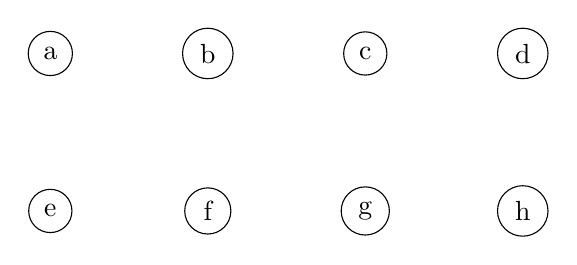
\begin{tikzpicture}
      \node[draw, circle] (a) at (0, 0) {a};
      \node[draw, circle] (b) at (2, 0) {b};
      \node[draw, circle] (c) at (4, 0) {c};
      \node[draw, circle] (d) at (6, 0) {d};
      \node[draw, circle] (e) at (0, -2) {e};
      \node[draw, circle] (f) at (2, -2) {f};
      \node[draw, circle] (g) at (4, -2) {g};
      \node[draw, circle] (h) at (6, -2) {h};
      % TODO: draw graph
    \end{tikzpicture}
    \caption{Gerichteter Graph $G$}
  \end{figure}

  Zeichnen Sie den entstehenden Tiefensuchwald. Geben Sie außerdem für alle Knoten $u \in V$ die berechneten Knoteneigenschaften $d(u)$ \& $f(u)$ am Ende des Algorithmus an.
\end{exercise}

\setcounter{subsection}{2}
\begin{eexercises}{Hashing}{
    Es seien die Hashfunktionen $h_1$ \& $h_2$ wie folgt definiert:
    \begin{align*}
      h_1(x) & = (3x + 5) \mod 7 \\
      h_2(x) & = (4x + 6) \mod 8
    \end{align*}
  }
  \item Illustrieren Sie die Hashatabelle der Größe 7, die entsteht, wenn zur Einfügung aller Elemente aus $K = \{1, 2, 4, 16, 20, 23, 26\}$ nacheinander in der angegebene Reihenfolge mit Hilfe von $h_1$ eingefügt werden.
  \item Illustrieren Sie die Hashatabelle der Größe 8, die entsteht, wenn zur Einfügung aller Elemente aus $K = \{1, 2, 4, 16, 20, 23, 26\}$ nacheinander in der angegebene Reihenfolge mit Hilfe von $h_2$ eingefügt werden
  \item Geben Sie jeweils für $h_1$ \& $h_2$ an, ob es sich um eine gute Wahl zur Konstruktion einer Hashtabelle mittels geschlossener Adressierung handelt oder nicht. Begründen Sie Ihre Aussage.
\end{eexercises}

\begin{eexercises}{O-Notation}{
  Jede der folgenden Teilaufgaben spezifiziert zwei Funktionen $f(n)$ \& $g(n)$. Bestimmen Sie jeweils, ob die vier Relationen $f(n) = \mathcal{O}(g(n)), f(n) = \mathcal{O}(g(n)), f(n) = \Omega(g(n)), f(n) = \omega(g(n))$ gelten (es sind also pro Teilaufgabe vier Antworten zu geben). Beweisen Sie Ihre Antwort jeweils kurz. Nutzen Sie dazu die Eigenschaften der asymptotischen Landau-Notation aus der Vorlesung (wie z.B. die ursprüngliche Definition, die Charakterisierung über Grenzwerte oder die darauffolgenden Lemmata).
    \hint{Die Basis des Logarithmus ist 2.}
    }
    \item $f(n) = 2n^2 + 23n^{3/2} + \log{n} -42$ und $g(n) = n^{2.001}$
    \item $f(n) = n \cdot (1 + (-1)^n)$ und $g(n) = 2n$
    \item $f(n) = 2\sqrt{n}$ und $g(n) = (3/2)^n$
    \item $f(n) = \sum_{i=1}^n \log{i}$ und $g(n) = n \log{n}$
\end{eexercises}

\begin{eexercises}{Algorithmenentwurf}{
    Gegeben sei ein ungerichteter, zusammenhängender Graph $G = (V, E)$. Ein Knoten $u \in V$ heißt Nadelöhr, wenn der Graph $G - u = (V \setminus \{u\}, E \setminus \{(v, w) \in E | v = u \lor w = u\})$ unzusammenhängend ist. Abbildung 2 zeigt ein Beispiel eines Graphen mit Nadelöhr.
  }
  \item Beschreiben Sie einen Algorithmus (als Pseudocode oder in Textform), der bei Eingabe eines ungerichteten, zusammenhängenden Graphen $G$ in Adjazenzlistendarstellung bestimmt, ob $G$ ein Nadelöhr besitzt. Ihr Algorithmus sollte Laufzeit $\bigO(|V| + |V| \cdot |E|)$ haben.
  \item Analysieren Sie die Laufzeit Ihres Algorithmus.
  \item Beweisen Sie die Korrektheit Ihres Algorithmus.
\end{eexercises}

\begin{eexercises}{Algorithmenentwurf II}{
    Entwerfen Sie anhand der folgenden Arbeitsschritte einen Divide \& Conquer Algorithmus, der bei Eingabe zweier natürlicher Zahlen $x \in \mathbb{N}$ und $n \in \mathbb{N}$ die Potenz
    \begin{equation*}
      x^n = x \cdot x \cdot \ldots \cdot x
    \end{equation*}
    in Laufzeit $\bigO(\log n)$ berechnet. Als arithmetische Operationen mit konstanter Laufzeit sind dabei lediglich die Addition, Subtraktion sowie Multiplikation zweier ganzer Zahlen erlaubt. Auch die Abfrage ob eine Zahl gerade oder ungerade ist, kann in konstanter Laufzeit erfolgen.
  }
  \item Beschreiben Sie Ihre algorithmische Idee zunächst informell.
  \hint{Überlegen Sie sich eine rekursive Formulierung für $x^n$ und erklären Sie, wie Ihr Algorithmus diese nutzt. Achten Sie darauf, dass die rekursive Formulierung die geforderte Laufzeitschranke ermöglicht.}
  \item Formulieren Sie Ihren Algorithmus in Pseudocode.
  \item Geben Sie die Laufzeit Ihres Algorithmus als Rekursionsgleichung an.
  \item Analysieren Sie die Laufzeit Ihres Algorithmus möglichst genau in der $\bigO$-Notation mit Hilfe der Substitutionsmethode. Sie können dabei annehmen, dass $n$ eine Zweierpotenz ist. Sollten Sie keine Lösung zu 3. haben, dürfen Sie stattdessen die Rekursionsgleichung $T(n) = 3 \cdot T(n/3) + 42$ mit $T(1) = 23$ auflösen.
  \hint{Ein Induktionsbeweis der Laufzeit ist nicht notwendig, aber aus Ihrer Rechnung muss klar hervorgehen, wie Sie zu Ihrer Lösung kommen.}
\end{eexercises}

\begin{eexercises}{Dynamische Programmierung}{
    Das Unternehmen Alset möchte aus $n$ verschiedenen Prototypen eines neuen elektrischen Traktors eine möglichst große Teilmenge realisieren. Die Realisierung von Protoyp $i$ verursacht Kosten $c_i \in \mathbb{N}$. Zur Umsetzung der ausgewählten Prototypen steht ein Budget $B \in \mathbb{N}$ zur Verfügung, welches die Kosten aller ausgewählten Prototypen decken muss.
  }
  \item Sei $\text{OPT}(i, b)$ die maximale Anzahl der ersten $i \in \{0, 1, \ldots, n\}$ Prototypen, die mit dem Budget $b \in \{0, 1, \ldots, B\}$ realisierbar sind. Finden Sie eine rekursive Formulierung für $\text{OPT}(i, b)$ und begründen Sie kurz deren Korrektheit.
  \hint{Nutzen Sie zur Lösung dieser Teilaufgabe ein aus der Vorlesung bekanntes Problem, welches die obige Situation modelliert.}
  \item Zur Realisierung von Prototyp $i$ müssen nun zusätzlich $m_i \in \mathbb{N}$ Mitarbeiter bereitgestellt werden. Es stehen insgesamt $M \in \mathbb{N}$, von denen jeder bei der Umsetzung von höchstens einem (beliebigen) Prototypen helfen kann. Entwickeln Sie eine rekursive Formulierung für die maximale Anzahl realisierbarer Projekte unter diesen zusätzlichen Randbedingungen \& begründen Sie kurz deren Korrektheit. Beachten Sie dabei die Laufzeitanforderung aus 3.
  \item Beschreiben Sie in Pseudocode einen Algorithmus, der mittels dynamischer Programmierung in Zeit $\bigO(n \cdot B \cdot M)$ die maximale Anzahl realisierbarer Projekte, unter Berücksichtigung des Gesamtbudgets und der verfügbaren Mitarbeiter, bestimmt. Die konkrete Teilmenge der zugehörigen Prototypen muss nicht bestimmt werden. Als Eingabe erhält Ihr Algorithmus die Werte $B$ und $M$ sowie die $n$-elementigen Arrays $c = [c_1, \ldots, c_n]$ und $m = [m_1, \ldots, m_n]$.
\end{eexercises}

\begin{eexercises}{Algorithmenentwurf III}{
    Um den Netzausbau in Deutschland voran zu treiben, hat sich der Telekommunikationsanbieter Mokelet dazu entschlossen, jedes Haus in dem Dorf Hintertupfingen mit 5G-Empfang zu versorgen. In Hintertupfingen gibt es genau $n \in \mathbb{N}$ Häuser, die alle entlang einer schnurgeraden, $k \in \mathbb{N}$ Kilometer langen Straße stehen. Um ein Haus mit 5G-Empfang zu versorgen, muss Mokelet 5G-Masten entlang der Straße aufstellen. Ein einzelner 5G-Mast kann beliebig viele Häuser in einer Entfernung bis zu 3 Kilometer versorgen. Da Hintertupfingen nur spärlich besiedelt ist, muss Mokelet genau planen, wo die teuren 5G-Masten errichtet werden sollen.\par
    Wir modellieren die Straße als Strecke auf dem Zahlenstrahl zwischen 0 und $k$. Der Standort des $i$-ten Hauses kann als (rationale) Zahl $h_i \in [0, k]$ beschrieben werden. Masten können an beliebigen (rationalen) Punkten im Intervall $[0, k]$ errichtet werden.
    \hint{Die Lösung einer Strategie $A$, die 5G-Masten aufstellt, kann zum Beispiel als Folge von rationalen Zahlen $a_1 < a_2$ beschrieben mit $a_2 \in [0, k]$ beschreiben werden. Der $i$-te 5G-Mast wird dabei an Position $a_i$ errichtet.}
  }
  \item Wo wäre (im Hinblick auf eine optimale Lösung) ein geeigneter Standort für die 5G-Mast, der das erste ("am weitesten links liegende") Haus versorgt?
  \item Beschreiben Sie einen Greedy-Algorithmus, der bei Eingabe eines Arrays $H = [h_1, \ldots h_n]$ der $n$ Haus-Standorte (in aufsteigender Reihenfolge) und der Länge $k$ der Straße in Laufzeit $\bigO(n)$ die minimale Anzahl an 5G-Masten bestimmt, die zur vollständigen Versorgung von Hintertupfingen notwendig sind.
  \item Analysieren Sie die Laufzeit Ihres Algorithmus.
  \item Beweisen Sie, dass Ihr Algorithmus eine optimale Lösung liefert.
\end{eexercises}



\sheet[20211]{Ersttermin}
\begin{exercises}{Big-O Notation}
\item Sei $f(n) = 23 \cdot n^{\log_2{9}}$. Nennen Sie zwei Funktionen $g_1(n)$ und $g_2(n)$, so dass die folgenden Eigenschaften erfüllt sind:
\begin{itemize}
  \item $g_1$ und $g_2$ wachsen asymptotisch echt schneller als $f$
  \item $g_1$ und $g_2$ wachsen nicht polynomiell schneller als $f$
  \item $g_1$ und $g_2$ wachsen asymptotisch nicht gleich schnell
\end{itemize}
Begründen Sie kurz, warum Ihre gewählten Funktionen die geforderten Eigenschaften erfüllen.
\item Entscheiden Sie, ob die folgenden Aussagen über Funktionen der Form $f: \mathbb{N} \to \mathbb{R}$ wahr oder falsch sind und beweisen bzw. widerlegen Sie diese. Falls Sie bekannte Rechenregeln aus der Vorlesung benutzen, so nennen Sie diese beim Namen bzw. referenzieren Sie diese.
\begin{itemize}
  \item $\log n = \bigO(\sqrt{n})$
  \item $\sum_{i=1}^n 3i - 7 = \Theta(n^2)$
  \item $\frac{n^2\cdot 2\sqrt{n})^3}{n^3-3} = \Omega(n) $
  \item $\prod_{i=1}^n (i + n) = \bigO(n^{2n})$
\end{itemize}
\end{exercises}

\begin{exercises}{Master-Theorem}
\item Entscheiden Sie, ob die folgende Rekursionsgleichung mithilfe des Mastertheorems lösbar ist oder nicht. Ist das Mastertheorem anwendbar, so lösen Sie die Rekursionsgleichung damit. Ist das Mastertheorem nicht anwendbar, so lösen Sie die Rekursionsgleichung mit der Substitutionsmethode.
\begin{equation*}
  T(n) = \begin{cases}
    2\cdot T(n/8)+\sqrt{n} & \text{für } n > 1 \\
    17                     & \text{sonst}
  \end{cases}
\end{equation*}
\item Für die Laufzeit $T(n)$ eines Algorithmus $A$ gelte die Rekursion
\begin{equation*}
  T(n) \leq \begin{cases}
    \max_{1\leq k\leq n}(3T(k-1)+T(n-k))+2\cdot n^2 & \text{für } n > 0 \\
    1                                               & \text{sonst}
  \end{cases}
\end{equation*}
Bestimmen und beweisen Sie eine möglichst exakte obere Schranke (im $\bigO$-Kalkül) für die Laufzeit von Algorithmus $A$.
\hint{Raten Sie eine Lösung \& verifizieren Sie diese dann durch vollständige Induktion.}
\end{exercises}

\begin{exercise}{Mergesort}
  Sortieren Sie das Array $A = [13,11,5, -1,3,0,42,1]$ durch Anwendung des Algorithmus MERGESORT aus der Vorlesung. Zur Erinnerung finden Sie Teile des zugehörigen Pseudocodes in Algorithmus 1. Geben Sie den Inhalt des Arrays $A$ nach jeder Durchführung der Merge-Operation in Zeile 5 an.
  \begin{algorithm}[ht]
    \caption{MERGESORT($A, l, r$)}
    \KwData{$A = [A[1], \ldots, A[n]]$}
    \KwResult{$A$ sortiert}
    \If{$l < r$}{
      $p \gets \lfloor (l + r)/2 \rfloor$ \\
      MERGESORT($A, l, p$) \\
      MERGESORT($A, p + 1, r$) \\
      MERGE($A, l, p, r$)
    }
  \end{algorithm}
\end{exercise}

\begin{eexercises}{Algorithmenentwurf}{
    Für ein Array $A[1, \ldots, n]$ von $n \in \mathbb{N}$ ganzen Zahlen nennen wir ein Index-Paar $(i, j)$ verdreht, wenn $i < j$ und $A[i] < A[j]$.
  }
  \item Geben Sie ein Array $A$ bestehend aus vier Zahlen und der kleinstmöglichen Anzahl an verdrehten Index-Paaren an. Um wieviele verdrehte Index-Paare handelt es sich genau?
  \item Geben Sie ein Array $A$ bestehend aus vier Zahlen und der größtmöglichen Anzahl an verdrehten Index-Paaren an. Um wieviele verdrehte Index-Paare handelt es sich genau?
  \item Geben Sie ein Array $A$ bestehend aus vier Zahlen und exakt drei verdrehten Index-Paaren an.
  \item Entwerfen Sie einen rekursiven Algorithmus, der bei Eingabe eines Array $A$ von $n$ ganzen Zahlen in Zeit $\mathcal{O}(n \log n)$ die Anzahl an verdrehten Index-Paaren bestimmt. Sie dürfen Pseudocode angeben, müssen es aber nicht. Sollte Ihr Algorithmus auf bekannten Algorithmen aus der Vorlesung basieren, reicht es die notwendigen Änderungen (klar \& deutlich!) zu beschreiben.
  \item Beweisen Sie, dass Ihr Algorithmus die geforderte Laufzeitschranke einhält.
\end{eexercises}

\begin{exercises}{Suchbäume}
\item Wählen Sie sechs unterschiedliche Zahlen mit Werten zwischen 0 und 50. In welcher Reihenfolge müssen Ihre gewählten Zahlen in einen (anfangs leeren) binären Suchbaum eingefügt werden, damit dieser maximal unbalanciert ist? Zeichnen Sie den resultierenden binären Suchbaum.
\item Wählen Sie sechs (neue) unterschiedliche Zahlen mit Werten zwischen 0 und 50. In welcher Reihenfolge müssen Ihre gewählten Zahlen in einen (anfangs leeren) binären Suchbaum eingefügt werden, damit dieser minimal unbalanciert ist? Zeichnen Sie den resultierenden binären Suchbaum.
\item Gegeben sei ein AVL-Baum für die Schlüssel $\{17,19,21,23,42,45,47,53,66\}$. Der Zustand der Datenstruktur ist in Abbildung 1 dargestellt. Löschen Sie das Element mit Schlüssel 42 gemäß der Löschoperation für AVL-Bäume aus der Vorlesung. Geben Sie dabei den Zustand der Datenstruktur nach jedem Entfernen eines Knotens und nach jeder Rotation an.
% TODO: insert avl tree
\end{exercises}

\begin{eexercises}{Dynamische Programmierung}{
    Betrachten Sie ein eindimensionales Gitter aus $n$ Feldern nummeriert von 1 bis $n$. Die kleine Ameise Esiema startet auf Feld 1. Befindet sich Esiema auf einem Feld am Rand (Feld 1 oder $n$), so bewegt sie sich im nächsten Schritt mit Wahrscheinlichkeit 1 in die freie Richtung (weg vom Rand). Befindet sich Esiema auf einem anderen Feld, so bewegt sie sich im nächsten Schritt mit Wahrscheinlichkeit 1/2 um ein Feld nach links und mit Wahrscheinlichkeit 1/2 um ein Feld nach rechts.
  }
  \item Abbildung 2 zeigt einen Ausschnitt der Tabelle mit den Wahrscheinlichkeiten, dass Esiema nach $i$ Schritten auf Feld $x$ ist. Ergänzen Sie die sechs fehlenden Werte für $x \in \{1,2,\ldots,6\}$ und $i = 5$. Sie können die fehlenden Werte direkt in die Tabelle eintragen oder auf eigenes Papier schreiben.
  \begin{tabular}{c|cccc ccc}
    $i \backslash x$ & 1      & 2      & 3      & 4      & 5      & 6      & \ldots \\
    \hline
    0                & 1      & 0      & 0      & 0      & 0      & 0      & \ldots \\
    1                & 0      & 1      & 0      & 0      & 0      & 0      & \ldots \\
    2                & 1/2    & 0      & 1/2    & 0      & 0      & 0      & \ldots \\
    3                & 0      & 3/4    & 0      & 1/4    & 0      & 0      & \ldots \\
    4                & 3/8    & 0      & 1/2    & 0      & 1/8    & 0      & \ldots \\
    5                &        &        &        &        &        &        & \ldots \\
    \ldots           & \ldots & \ldots & \ldots & \ldots & \ldots & \ldots & \ldots \\
  \end{tabular}
  \item Betrachten Sie ein zweidimensionales Array (Tabelle) $D$ der Größe $(n + 1) \times n$. Ein Eintrag $D[i,x]$ für $i \in \{0,1,\ldots,n\}$ und $x \in \{1,2,\ldots,n\}$ entspricht dabei der Wahrscheinlichkeit, dass Esiema nach $i$ Schritten auf Feld $x$ ist. Entwerfen Sie eine Rekursion zum Berechnen von $D$ und begründen Sie kurz (!) in Worten die Korrektheit der Rekursion.
  \item Geben Sie einen Algorithmus in Pseudocode an, der mittels dynamischer Programmierung bestimmt, auf welchen Feldern sich Esiema nach $n$ Schritten mit der größten Wahrscheinlichkeit aufhält.
\end{eexercises}

\begin{eexercises}{Algorithmenentwurf II}{
    Nach Ihrem Informatik-Studium starten Sie als Comedian durch. Sie sind sehr erfolgreich und haben bald mehr Anfragen als Sie annehmen können. Jede Anfrage besteht aus einer angebotenen Gage (in Euro) und einer Deadline (in Tagen), bis zu der der Auftritt erfolgen muss. Aus zeitlichen Gründen können Sie pro Tag maximal einen Auftritt absolvieren. Sie wollen eine Teilmenge von Anfragen annehmen, die Ihre Einnahmen maximiert. Sie erinnern sich an Ihr Informatik-Studium und entwerfen einen gierigen Algorithmus, der dieses Problem optimal in polynomieller Zeit löst. Als Eingabe erhält Ihr Algorithmus zwei Arrays $G$ und $D$ mit jeweils $n \in \mathbb{N}$ Elementen. Der Eintrag $G[i] > 0$ entspricht der Gage die Sie bei der $i$-ten Anfrage erhalten. Der Eintrag $D[i] > 0$ entspricht der Deadline der $i$-ten Anfrage.
    \hint{zB. seien ihre aktuellen Anfragen gegeben durch 1. Gage: 100€, Deadline: 2 Tage 2. Gage: 200€, Deadline: 2 Tage 3. Gage: 300€, Deadline: 1 Tag 4. Gage: 50€, Deadline: 1 Tag. Eine optimale Auswahl an Anfragen wären Anfragen 2 und 3 für insgesamt 500€.}
  }
  \item Welches Angebot sollte Ihr Algorithmus zuerst akzeptieren und an welchem Tag sollte der zugehörige Auftritt stattfinden? Welches Angebot sollte Ihr Algorithmus als zweites akzeptieren und an welchem Tag sollte der zugehörige Auftritt stattfinden? Begründen Sie diese Wahlen kurz (!) in Worten.
  \item Beschreiben Sie die allgemeine Vorgehensweise des gierigen Algorithmus kurz in Worten.
  \item Geben Sie Ihren Algorithmus in Pseudocode an. Der Algorithmus soll die Indizes der auszuwählenden Anfragen sowie die dadurch erzielten Einnahmen ausgeben.
\end{eexercises}



\sheet[20212]{Zweittermin}
\begin{eexercises}{Big-O Notation}{
    Entscheiden Sie, ob die folgenden Aussagen über Funktionen der Form $N \to R$ wahr oder falsch sind und beweisen bzw. widerlegen Sie diese. Falls Sie bekannte Rechenregeln oder Resultate aus der Vorlesung benutzen, so nennen Sie diese beim Namen bzw. referenzieren Sie diese.
    \hint{Der Ausdruck $\log n$ bezeichnet den Logarithmus von $n$ zur Basis 2. Der Ausdruck $\ln n$ bezeichnet den Logarithmus von $n$ zur Basis $e$.}
  }
  \item $n^2\cdot \ln{n} = o(n^{3/2}\cdot \log{n})$
  \item $\frac{(2n^2)\cdot \sqrt{n^5}}{n^{3.5}+n^2} = \Omega{0.001\cdot n}$
  \item $2^n = \Theta(2^{n/2})$
  \item $\sum_{i=1}^n \log{i} = \bigO(2n\cdot \log{n})$
\end{eexercises}

\begin{exercises}{Master-Theorem}
\item Geben Sie eine Funktion $f$ an, so dass auf die Rekursion $T(n) \leq 4 \cdot T(n/2) + f(n)$ keiner der drei Fälle des Master-Theorems angewendet werden kann. Begründen Sie Ihre Antwort!
\item Entscheiden und begründen Sie, ob die folgende Rekursionsgleichung mithilfe des Mastertheorems lösbar ist oder nicht. Ist das Mastertheorem anwendbar, so lösen Sie die Rekursionsgleichung damit. Ist das Mastertheorem nicht anwendbar, so lösen Sie die Rekursionsgleichung mit der Substitutionsmethode.
\begin{equation*}
  T(n) = \begin{cases}
    9 \cdot T(n/\log_{1/2}(1/8)) + n^3 & \text{für } n > 1 \\
    1                                  & \text{sonst}
  \end{cases}
\end{equation*}
\hint{Sollten Sie die Substitutionsmethode nutzen, müssen Sie in dieser Teilaufgabe nicht noch zusätzlich einen Induktionsbeweis zur Korrektheit aufführen.}
\item Sei $T(n)$ die Laufzeit eines gegebenen Algorithmus $A$. Für diese Laufzeit gelte die folgende rekursive obere Schranke:
\begin{equation*}
  T(n) \leq \begin{cases}
    1/3                & \text{für } n \leq 1 \\
    3 \cdot T(n-2) + 3 & \text{sonst}
  \end{cases}
  % T(n) \leq \frac{1}{3}, \text{ für } n \leq 1, 3 \cdot T(n-2) + 3, \text{ sonst}
\end{equation*}
\item Bestimmen und beweisen Sie eine möglichst exakte (nicht-rekursive) obere Schranke (im $\bigO$-Kalkül) für die Laufzeit von Algorithmus $A$.
\hint{Raten Sie eine Lösung der Rekursion und beweisen Sie deren Korrektheit durch vollständige Induktion. Beim Raten der Lösung muss ersichtlich werden, wie Sie zu der geratenen Lösung gekommen sind (z.B. durch Angabe der zugehörigen Rechnung beim Anwenden der Substitutionsmethode).}
\end{exercises}

\begin{exercise}{Quicksort}
  Sortieren Sie das Array $A = [13,11,5, -1,3,0,42,1]$ durch Anwendung des Algorithmus QUICKSORT aus der Vorlesung. Zur Erinnerung finden Sie die zugehörigen Pseudocodes als Algorithmen 1 \& 2. Geben Sie den Inhalt des Arrays $A$ nach vollständigen Ausführung des PARTITION-Aufrufs in Zeile 2 von Algorithmus 1 an.
  \begin{algorithm}[ht]
    \caption{QUICKSORT($A, l, r$)}
    \KwData{$A = [A[1], \ldots, A[n]]$}
    \KwResult{$A$ sortiert}
    \If{$l < r$}{
      $p \gets \text{PARTITION}(A, l, r)$ \\
      QUICKSORT($A, l, p - 1$) \\
      QUICKSORT($A, p + 1, r$)
    }
  \end{algorithm}
\end{exercise}

\begin{eexercises}{Graphen}{
    Wir wollen die zuverlässigsten Kommunikationswege zwischen je zwei Computern in einem gegebenen Computer-Netzwerk ermitteln. Dazu sei das Computer-Netzwerk Abbildung 1 zeigt als Beispiel den Graphen zu dem Computer-Netzwerk der (sehr kleinen) Universität Grubmah.
    % TODO: insert graph
  }
  \item Betrachten Sie den Graphen in Abbildung 1. Nennen Sie einen Pfad von g nach d mit der höchsten Zuverlässigkeit \& geben Sie die entsprechende Zuverlässigkeit an. Nennen Sie außerdem einen kreisfreien Pfad von g nach d mit der niedrigsten Zuverlässigkeit und geben Sie die entsprechende Zuverlässigkeit an.
  \item Entwerfen Sie einen Algorithmus, der einen zuverlässigsten Pfad von einem gegebenen Computer zu einem anderen gegebenen Computer in Laufzeit $\bigO(|V| \cdot \log|V| + |E| \cdot \log|V|)$ findet. Sie dürfen Pseudocode angeben, müssen es aber nicht. Sollte Ihr Algorithmus auf bekannten Algorithmen aus der Vorlesung basieren, reicht es die notwendigen Änderungen (klar und deutlich!) zu beschreiben.
  \item Analysieren Sie die Laufzeit Ihres Algorithmus.
\end{eexercises}

\begin{eexercises}{UNION-FIND Datenstruktur}{
    Wir betrachten die Datenstruktur für disjunkte dynamische Mengen wie in der Vorlesung definiert. Die Grundmenge (das Universum) sei $U = \mathbb{Z}$, also die Menge aller ganzen Zahlen.
    % TODO: insert visualisation
  }
  \item Wählen Sie eine Menge $A$ von $|A| = 8$ unterschiedlichen Zahlen mit Werten zwischen 50 und 50. Geben Sie eine Folge von Aufrufen der Operationen MAKE-SET und UNION an, welche die von Ihnen gewählten Zahlen in drei disjunkte Mengen $A_1, A_2$ und $A_3$ aufteilt, so dass $|A_1| = 3, |A_2| = 4$ und $|A_3| = 1$ gilt.
  \item Skizzieren Sie die zwei Mengenobjekte für $A_1$ und $A_2$, nachdem die disjunkten Mengen gemäß Ihrer Lösung zu Punkt (a) erzeugt wurden. Eine mögliche Darstellung eines Mengenobjektes ist in Abbildung 2 zu sehen.
  \item Seien $M := \max A$ und $m := \min A$ jeweils die maximale und minimale der von Ihnen in Punkt (a) gewählten Zahlen. Geben Sie die Rückgabewerte der Aufrufe FIND-SET($M$) und FIND-SET($m$) an, nachdem die disjunkten Mengen gemäß Ihrer Lösung zu Punkt (a) erzeugt wurden.
  \item Geben Sie zwei verschiedene Aufrufe an, welche die beiden zu $A_1$ und $A_2$ gehörigen Mengenobjekte aus Punkt (a) zu einem neuen Mengenobjekt vereinigen. Geben Sie außerdem für einen der beiden Aufrufe an, in welcher Reihenfolge die Zahlen in der Liste des erzeugten Mengenobjektes gespeichert sind.
\end{eexercises}

\begin{eexercises}{Dynamische Programmierung}{
    Früh am Ostersonntag fehlt dem Osterhasen nur noch Hamburg, bevor er endlich in den wohlverdienten Feierabend kann. Leider befindet er sich auf der falschen Seite der Elbe und der Elbtunnel ist gesperrt. Glücklicherweise findet er eine Stelle, an der die beiden Ufer der Elbe über eine Reihe von $n$ Holzpfählen modelliert als Kantengewichten zuverlässig verbunden sind. Die Holzpfähle sind unterschiedlich hoch: der $i$-te Pfahl vom Ufer aus hat Höhe $h_i > 0$. Der Osterhase kann – als geübter Hoch- und Weitspringer – vom $i$-ten Pfahl entweder auf Pfahl $i+1$ oder Pfahl $i+2$ springen. Springt er von Pfahl $i$ nach Pfahl $j \in \{i + 1, i + 2\}$, verliert er leider immer $|h_i - h_j|$ Ostereier. Kurzentschlossen zückt der Osterhase sein Handy, ruft Sie als Experten für Elbüberquerungen auf Holzpfählen an und bittet Sie darum, ihm zu helfen von Pfahl 1 nach Pfahl $n$ zu kommen und dabei möglichst wenige Ostereier zu verlieren.
  }
  \item Angenommen, Sie wissen für jeden der ersten vier Pfähle, wie Sie unter dem geringsten Verlust an Ostereiern von Pfahl 1 zu dem jeweiligen Pfahl kommen. Beschreiben Sie in Worten ein rekursives Vorgehen, um mit diesem Wissen unter dem geringsten Verlust an Ostereiern von Pfahl 1 zu Pfahl 5 zu kommen.
  \item Geben Sie aufbauend auf Ihrer Rekursion aus Punkt 1. eine vollständige mathematische Rekursionsformel für die geringste Anzahl an verlorenen Eiern zum Erreichen von Pfahl $i \in \{1, 2, \ldots, n\}$ an. Begründen Sie kurz in Worten die Korrektheit Ihrer Rekursionsformel.
  \item Geben Sie einen Algorithmus in Pseudocode an, der miiels dynamischer Programmierung besXmmt, in welcher Reihenfolge der Osterhase auf welche Pfähle springen muss, um die Elbe mit einem möglichst geringen Verlust an Ostereiern zu überqueren.
\end{eexercises}

\begin{eexercises}{MERGE Algorithmus}{
    Gegeben seien $n$ jeweils aufsteigend sortierte Arrays $A_1, \ldots, A_n$. Unser Ziel ist es, alle $n$ Arrays durch wiederholte Anwendung des aus der Vorlesung bekannten Merge-Algorithmus zu einem einzigen aufsteigend sortierten Array zusammenzufügen. Im Folgenden gehen wir davon aus, dass Merge zwei aufsteigend sortierte Arrays $L$ und $R$ als Eingabe erhält und ein neues aufsteigend sortiertes Array $A$ mit allen Elementen aus $L$ und $R$ zurück gibt. Abgesehen davon funktioniert Merge wie in der Vorlesung beschrieben.
  }
  \item Zur Erzeugung des Arrays $A$ muss Merge jeweils Elemente aus den Eingabearrays $L$ und $R$ miteinander vergleichen. Wie viele solcher Vergleiche führt Merge bei Eingabe zweier Arrays der Längen $l$ und $l'$ durch? Begründen Sie Ihre Antwort.
  \item Beschreiben Sie einen gierigen Algorithmus, der die $n$ aufsteigend sortierten Eingabearrays $A_1, \ldots, A_n$ zu einem einzigen, aufsteigend sortierten Array zusammen fügt. Ihr Algorithmus darf die gegebenen/erzeugten Arrays nicht direkt verändern sondern muss dazu ausschließlich Merge-Aufrufe verwenden. Dabei soll ihr Algorithmus die Gesamtzahl der Vergleiche in allen Merge-Aufrufen minimieren. Sie dürfen Pseudocode verwenden, müssen es allerdings nicht.
  \hint{Es dürfen auch nicht benachbarte Arrays zusammengefügt werden.}
  \item Beweisen Sie, dass Ihr Algorithmus aus Punkt (b) die Gesamtzahl der Vergleiche in allen Merge-Aufrufen minimiert.
\end{eexercises}



\sheet[2022]{Ersttermin}
\begin{exercises}{Algorithmen}
\item Betrachten Sie folgenden Algorithmus in ihrer aus der Vorlesung bekannten Implementierung. Wählen Sie geeignete Parameter zur Beschreibung der Eingabegröße und nutzen Sie diese, um eine möglichst gute obere Schranke an die asymptotische Laufzeitkomplexität (worst-case) anzugeben.
\hint{Beispiel PRIM: $n$ Anzahl Knoten, $m$ Anzahl Kanten $\to$ Laufzeit $\mathcal{O}(n \cdot \log^2(n) + m \cdot \log(n))$}
\begin{itemize}
  \item QUICKSORT
  \item COUNTINGSORT
  \item DIJKSTRA (single-source shortest path)
  \item FLOYD-WARSHALL (all-pairs shortest path)
\end{itemize}
\item Wann ist ein Sortieralgorithmus stabil? Nennen Sie einen stabilen Sortieralgorithmus aus der Vorlesung.
\item Wie wurden die folgenden Begriffe in der Vorlesung definiert?
\begin{itemize}
  \item polynomialzeit-berechenbar
  \item polynomialzeit-verifizierbar
\end{itemize}
\end{exercises}

\begin{exercise}{Heapsort}
  Das Array $A = [2,3,4,9,6,5]$ soll mit Hilfe des in der Vorlesung vorgestellten HEAPSORT Algorithmus aufsteigend sortiert werden. Zur Erinnerung finden Sie Teile des Pseudocodes in Algorithmen 1 \& 2. Geb
  \begin{algorithm}[ht]
    \caption{HEAPSORT($A$)}
    \KwData{$A = [A[1], \ldots, A[n]]$}
    \KwResult{$A$ sortiert}
    BUILDHEAP($A$) \\
    \For{$i \gets n$ \textbf{downto} 2}{
      DELETEMAX($A$)
    }
  \end{algorithm}
\end{exercise}

\begin{exercises}{O-Notation}
\item Ordnen Sie die folgenden Funktionen aufsteigend gemäß ihres asymptotischen Wachstums (ohne Begründung):
\begin{equation*}
  n^5,\sqrt{n},n^{1/3},n!,1/100,\sqrt{2^n},n,\log_3(n),n/\log_2{n},16^{\log_2{n}}
\end{equation*}
\item Berechnen Sie für die folgenden Funktionen scharfe Schranken in möglichst einfacher Darstellung der $\bigO$- \& $\Omega$-Notation. Ihr Rechenweg muss nachvollziehbar sein. Sie dürfen auf die aus der Vorlesung bekannten Eigenschaften der $\bigO$- \& $\Omega$-Notation zurückgreifen.
\begin{align*}
  f(n) = 42\log_2(n) + 23\sqrt{n} + n^{1/16} \\
  g(n) = n^{3+\cos{\frac{n\pi}{2}}}
\end{align*}
\item Beweisen oder widerlegen Sie:\par Für zwei nicht-negative Funktionen $f_1, f_2: \mathbb{N} \to \mathbb{R}$ gilt immer $f_1(n) = \bigO(f_2(n))$ oder $f_1(n) = \Omega(f_2(n))$.
\end{exercises}

\begin{exercises}{Master-Theorem}
\item Geben Sie eine Funktion $f$ an, so dass auf die Rekursion
\begin{equation*}
  T(n) = \begin{cases}
    4\cdot T(n/2) + f(n) & \text{für } n > 1 \\
    1                    & \text{sonst}
  \end{cases}
\end{equation*}
keiner der drei Fälle des Master-Theorems angewendet werden kann. Begründen Sie Ihre Antwort!
\item Lösen Sie die folgende Rekursion mit Hilfe des Mastertheorems:
\begin{equation*}
  T(n) = \begin{cases}
    3\cdot T(n/9) + n & \text{für } n > 1 \\
    1                 & \text{sonst}
  \end{cases}
\end{equation*}
\end{exercises}

\begin{eexercises}{Algorithmenanalyse}{
    Betrachten Sie Algorithmus 3:
    \begin{algorithm}[ht]
      \caption{WHOAMI($a, b$)}
      $n \gets 0$ \\
      \For{$i \gets a$ \textbf{to} $b$}{
        $n \gets n + i$ \\
        \If{$a \mod 2 = 1$}{
          $a \gets a + 1$
        }
        \If{$b \mod 2 = 1$}{
          $b \gets b - 1$
        }
        $m \gets 0$ \\
        $i \gets a$ \\
        \While{$i \leq b$}{
          $m \gets m + i$ \\
          $i \gets i + 2$
        }
      }
      \Return $n + m$
    \end{algorithm}
  }
  \item Geben Sie den Rückgabewert des Aufrufs WHOAMI(1,6) sowie den Inhalt der Variablen $a, b, n$ \& $m$ am Ende des Algorithmus an.
  \item Was berechnet Algorithmus 3 für die Eingabe $a, b \in \mathbb{N}$ mit $a < b$? Begründen Sie Ihre Antwort.
  \item Analysieren Sie die Laufzeit des Algorithmus in Abhängigkeit der Eingaben $a, b \in \mathbb{N}$ mit $a < b$ und begründen Sie ihre Antwort.
  \item Formulieren Sie eine sinvolle Invariante für den Wert der Variable $m$ zu Beginn eines Durchlaufs der While-Schleife mit dem Zählerwert $i$.
  \hint{Die Invariante muss geeignet sein, die Korrektheit von Algorithmus zu zeigen. Sie müssen die Korrektheit der Invariante/des Algorithmus nicht beweisen.}
\end{eexercises}

\begin{exercise}{Graphen}
  Sei $G = (V, E)$ ein kantengewichteter, ungerichteter Graph und $A \subseteq E$ eine Teilmenge der Kanten eines minimalen Spannbaums (MST) von $G$. Weiter sei $(C, V \setminus C)$ ein mit $A$ verträglicher Schnitt und $e = \{u, v\} \in E$ eine leichte Kante, die $(C, V \setminus C)$ kreuzt.\par
  Beweisen Sie: $A \cup \{e\}$ ist auch Teilmenge der Kanten eines MST von $G$.
\end{exercise}

\begin{eexercises}{Dynamische Programmierung}{
    Sie haben ein sehr langes, sehr schmales Rasenstück der Länge $l \in \mathbb{N}$ zu bewässern. Entlang des Rasenstücks sind $n \in \mathbb{N}$ Rasensprenger an den Positionen $0 \leq p_1 < \ldots < p_n \leq l$ platziert. Der Rasensprenger an Position $p_i$ hat Reichweite $r_i \geq 0$ in beide Richtungen entlang der langen Kante, so dass er den Rasen von Position $p_i - r_i$ bis Position $p_i + r_i$ (auf der gesamten Breite) bewässert. Wenn alle Rasensprenger eingeschaltet sind, wird der gesamte Rasen (von Position 0 bis Position $l$) bewässert. Ihre Aufgabe ist es, so wenig Rasensprenger wie möglich einzuschalten, damit der gesamte Rasen bewässert wird. Die Positionen \& Reichweiten der $n$ Rasensprenger sind als ganzzahlige Arrays $P = \langle p_1, \ldots, p_n \rangle$ und $R = \langle r_1, \ldots, r_n \rangle$ gegeben.
  }
  \item Betrachten Sie die Eingabe für ein Rasenstück der Länge $l = 7$ mit $n = 3$ Rasensprengern an den Positionen $P = \langle 1,3,6 \rangle$ und den zugehörigen Reichweiten $R = \langle 4,2,2 \rangle$. Welche Rasensprenger müssen Sie anschalten um den gesamten Rasen mit möglichst wenigen Rasensprengern zu bewässern?
  \item Betrachten Sie die folgende gierige algorithmische Idee: Schalte zunächst alle Rasensprenger aus. Schalte dann der Reihe nach die Rasensprenger ein, die die insgesamt bewässerte Fläche am meisten vergrößern, bis die gesamte Rasenfläche bewässert ist. Zeigen Sie, dass diese Strategie nicht optimal ist.
  \item Entwerfen Sie einen Algorithmus mittels dynamischer Programmierung für die Eingaben $l, P \& R$ die minimale Anzahl an notwendigen Rasensprengern in Zeit $\mathcal{O}(n \cdot l)$ zurückgibt ($n = \lvert P \rvert$). Geben Sie dazu zunächst eine geeignete mathematische Rekursionsgleichung an \& entwickeln Sie darauf aufbauend einen iterativen Algorithmus in Pseudocode.
  \hint{Bemerkung zu möglichem Ansatz für die Rekursion: Unterscheiden Sie die beiden Fälle, ob die optimale Lösung den letzten Rasensprenger einschaltet oder nicht.}
\end{eexercises}



\sheet[2023]{Probeklausur}

\end{document}